%% Journal of Computational Law and Legal Technology (Bon View Publishing)
%% REVISED version (manuscript #12050) of "LexFlip: A Dissociation Diagnostic
%% for Legal Meaning Preservation Metrics". Text revised in response to the
%% four reviews is set in blue through \rev{...}; the submitted version is
%% kept unchanged in jcllt_version.tex for comparison.
%%
%% Built from paper/main.tex with the analyses that main.tex defers to
%% paper/supplementary.tex folded into the body, since the journal takes no
%% appendix. Numbers come from paper/numbers.tex and the tables from
%% paper/tables/, which are the same files the preprint uses, so the two
%% versions cannot drift apart.
\documentclass{BVP_JCLLT}

%% The history dates and DOI are assigned by the editorial office at
%% production; the template's placeholders ("d month yyyy", "XXXXXXXX") are
%% left unset rather than printed, as the reviewers asked.

\OAText{{\copyright} The Author(s) 2026. Published by BON VIEW PUBLISHING PTE. LTD. This is an open access article under the CC BY License (https://creativecommons.org/licenses/by/4.0/).}

%% The class supplies booktabs-style rules under its own names. The shared
%% table files in tables/ are written against booktabs, so the one name that
%% differs is aliased rather than editing files main.tex also reads.
\let\bottomrule\botrule

%% BVP_JCLLT.cls closes the table* environment by resetting two switches it
%% never declares, so a full-width table raises "Undefined control sequence".
%% Declaring them here leaves the class file itself untouched.
\newif\iftablefootnotenone
\newif\ifkilltableabovespace

%% The class builds a table caption as "Table 1 " followed by the caption
%% punctuation, which prints a space before the full stop. Figure captions are
%% built without that space, so this only restores consistency between the two.
\makeatletter
\def\fnum@table{\tablename\ \thetable}
\makeatother

%% Give LaTeX more room to place the eleven floats next to the text that
%% discusses them; with the class defaults a full-width table is deferred and
%% the deferred floats collect on pages of their own.
\renewcommand{\topfraction}{0.92}
\renewcommand{\dbltopfraction}{0.92}
\renewcommand{\bottomfraction}{0.7}
\renewcommand{\textfraction}{0.06}
\renewcommand{\floatpagefraction}{0.85}
\renewcommand{\dblfloatpagefraction}{0.9}
\setcounter{topnumber}{3}
\setcounter{dbltopnumber}{1}
\setcounter{bottomnumber}{2}
\setcounter{totalnumber}{4}

%% Balances the two columns of the final page so the reference list ends level
%% instead of leaving one column half empty.
\usepackage{balance}

%% Columns end where their content ends rather than being stretched to full
%% height, which otherwise opens gaps between a float and the text under it.
\raggedbottom

%% Numeric macros for every figure quoted in the text, shared with main.tex.
\newcommand{\alphaOrd}{0.325}
\newcommand{\ceilR}{0.597}
\newcommand{\ceilRmse}{3.27}
\newcommand{\bestPairR}{0.606}
\newcommand{\meanPairR}{0.462}
\newcommand{\sbRel}{0.811}
\newcommand{\sbSqrt}{0.90}
\newcommand{\lenientMean}{7.61}
\newcommand{\strictMean}{4.34}
\newcommand{\medianRange}{7}
\newcommand{\pctSpreadSix}{63\%}
\newcommand{\labelSd}{2.40}
\newcommand{\testN}{89}
\newcommand{\mindetect}{0.73}
\newcommand{\annotMeans}{4.33, 7.57, 7.55, 7.72, 4.36}
\newcommand{\numedits}{373}
\newcommand{\numeditsTierOne}{310}
\newcommand{\meanjaccard}{0.93}
\newcommand{\minjaccard}{0.75}
\newcommand{\surfR}{0.62}
\newcommand{\maxMargin}{0.670}
\newcommand{\meanMargin}{0.172}
\newcommand{\nMetricsChallenged}{13}
\newcommand{\minMargin}{0.011}
\newcommand{\bertMargin}{0.039}
\newcommand{\simMarginLo}{0.022}
\newcommand{\partyMargin}{0.020}
\newcommand{\partyMarginLo}{0.006}
\newcommand{\partyMarginHi}{0.036}
\newcommand{\nParty}{14}
\newcommand{\partyMarginAll}{0.035}
\newcommand{\ruleMarginMeanSim}{0.029}
\newcommand{\dissocRho}{0.58}
\newcommand{\dissocRhoLo}{-0.08}
\newcommand{\dissocRhoHi}{0.90}
\newcommand{\nDissoc}{10}
\newcommand{\dissocRhoP}{0.08}
\newcommand{\dissocRhoAll}{0.24}
\newcommand{\dissocRhoAllLo}{-0.39}
\newcommand{\dissocRhoAllHi}{0.75}
\newcommand{\nDissocAll}{13}
\newcommand{\dissocRhoAllP}{0.43}
\newcommand{\isoDeltaR}{0.074}
\newcommand{\isoDeltaRho}{0.014}
\newcommand{\nliIdentRaw}{0.780}
\newcommand{\nliIdentPass}{1.3}
\newcommand{\nRules}{12}
\newcommand{\ruleMarginMean}{0.155}
\newcommand{\bestRuleMargin}{0.333}
\newcommand{\ruleSizeR}{0.25}
\newcommand{\ruleSizeLo}{-0.66}
\newcommand{\ruleSizeHi}{0.73}
\newcommand{\judgeR}{0.755}
\newcommand{\judgeRsd}{0.054}
\newcommand{\judgeRraw}{0.723}
\newcommand{\judgeRmse}{1.57}
\newcommand{\judgeMargin}{0.370}
\newcommand{\judgeMarginTierOne}{0.412}
\newcommand{\judgeDiscrim}{86.3}
\newcommand{\judgeIdent}{10.00}
\newcommand{\judgeEdit}{6.69}
\newcommand{\judgeEditTierOne}{6.31}
\newcommand{\judgeUnrel}{1.06}
\newcommand{\judgeAlphaSelf}{0.689}
\newcommand{\judgeKone}{0.611}
\newcommand{\judgeKfive}{0.719}
\newcommand{\judgeMeanRating}{9.11}
\newcommand{\judgeHumanR}{0.544}
\newcommand{\humanHumanR}{0.462}
\newcommand{\judgeAlphaPanel}{0.300}
\newcommand{\judgeErrEdit}{78.1}
\newcommand{\judgeErrIncoh}{54.6}
\newcommand{\judgeErrIdent}{0.0}
\newcommand{\judgeCalls}{7{,}080}
\newcommand{\judgeCost}{0.99}
\newcommand{\asymWeaken}{4.72}
\newcommand{\asymStrengthen}{8.02}
\newcommand{\asymGap}{3.30}
\newcommand{\asymWeakenN}{82}
\newcommand{\asymStrengthenN}{111}
\newcommand{\repRcalOne}{0.755}
\newcommand{\repRcalTwo}{0.726}
\newcommand{\repMarginOne}{0.370}
\newcommand{\repMarginTwo}{0.372}
\newcommand{\repItemR}{0.912}
\newcommand{\repProbeR}{0.982}
\newcommand{\repAsymOne}{3.30}
\newcommand{\repAsymTwo}{3.02}
\newcommand{\repNstats}{14}
\newcommand{\promptMarginLo}{0.421}
\newcommand{\promptMarginHi}{0.687}
\newcommand{\promptMarginRange}{0.267}
\newcommand{\promptRLo}{0.687}
\newcommand{\promptRHi}{0.758}
\newcommand{\nPrompts}{3}
\newcommand{\promptBareMargin}{0.687}
\newcommand{\promptBareR}{0.758}
\newcommand{\promptBareEdit}{3.83}
\newcommand{\promptRubricMargin}{0.421}
\newcommand{\promptRubricR}{0.687}
\newcommand{\promptRubricEdit}{6.25}
\newcommand{\reasonerR}{0.580}
\newcommand{\reasonerMargin}{0.320}
\newcommand{\chatKoneR}{0.619}
\newcommand{\chatKoneMargin}{0.425}
\newcommand{\asymGapLo}{3.24}
\newcommand{\asymGapHi}{4.03}
\newcommand{\nConfigs}{5}
\newcommand{\hybridR}{0.762}
\newcommand{\hybridMargin}{0.574}
\newcommand{\hybridW}{0.74}
\newcommand{\judgeCalMargin}{0.577}
\newcommand{\nliCalMargin}{0.549}

%% Numbers added in the revision (src/make_revision_tables.py).
\newcommand{\nliMarginNoBug}{0.685}
\newcommand{\nBugs}{12}
\newcommand{\maxBugShift}{0.015}
\newcommand{\expLexAgree}{102}
\newcommand{\expLexN}{112}
\newcommand{\expTOneAgree}{81}
\newcommand{\expTOneN}{85}
\newcommand{\expTTwoAgree}{21}
\newcommand{\expTTwoN}{27}
\newcommand{\expNeuAgree}{44}
\newcommand{\expNeuN}{44}
\newcommand{\expParAgree}{16}
\newcommand{\expParN}{44}
\newcommand{\expParChange}{19}
\newcommand{\expParUncertain}{9}
\newcommand{\expReverse}{26}
\newcommand{\expYes}{102}
\newcommand{\expLexUnidiom}{33}
\newcommand{\expCtrlUnidiom}{0}
\newcommand{\expCtrlN}{88}
\newcommand{\expTotal}{200}
\newcommand{\expBugsSample}{4}
\newcommand{\nSingular}{34}
\newcommand{\maxSingularShift}{0.032}
\newcommand{\nliMarginLo}{0.626}
\newcommand{\nliMarginHi}{0.721}
\newcommand{\judgeMarginLo}{0.336}
\newcommand{\judgeMarginHi}{0.402}
\newcommand{\nliMarginTone}{0.760}
\newcommand{\nliMarginTtwo}{0.228}
\newcommand{\judgeMarginTtwo}{0.158}
\newcommand{\simMarginTtwoLo}{0.005}
\newcommand{\simMarginTtwoHi}{0.034}
\newcommand{\judgeTies}{13.7}
\newcommand{\lenTies}{88.7}
\newcommand{\nliUnrelLo}{0.668}
\newcommand{\nliUnrelHi}{0.672}
\newcommand{\simUnrelLo}{0.021}
\newcommand{\simUnrelHi}{0.040}
\newcommand{\nUnrelDraws}{8}
\newcommand{\holmMaxP}{0.010}
\newcommand{\lenMinusFlau}{0.129}
\newcommand{\lenMinusFlauLo}{-0.026}
\newcommand{\lenMinusFlauHi}{0.289}
\newcommand{\lenRclLo}{0.55}
\newcommand{\lenRclHi}{0.66}
\newcommand{\lenRitLo}{0.54}
\newcommand{\lenRitHi}{0.68}
\newcommand{\nClusterSig}{9}
\newcommand{\powerRtwothree}{0.35}
\newcommand{\powerBelow}{0.14}
\newcommand{\powerAbove}{0.72}
\newcommand{\ceilTest}{0.599}
\newcommand{\ridgeRfour}{0.599}
\newcommand{\lenRfour}{0.628}
\newcommand{\judgeRfour}{0.738}
\newcommand{\flauRfour}{0.463}
\newcommand{\lenBucketLoSmall}{0.04}
\newcommand{\lenBucketHiSmall}{0.45}
\newcommand{\lenBucketLoMedium}{-0.02}
\newcommand{\lenBucketHiMedium}{0.34}
\newcommand{\lenBucketLoLarge}{0.47}
\newcommand{\lenBucketHiLarge}{0.68}
\newcommand{\labseMedLo}{0.37}
\newcommand{\labseMedHi}{0.67}
\newcommand{\flauMedLo}{0.29}
\newcommand{\flauMedHi}{0.59}
\newcommand{\judgeCallsTotal}{21{,}275}
\newcommand{\llamaCalls}{11{,}205}
\newcommand{\judgeCostTotal}{2.08}
\newcommand{\judgeDateFirst}{3~September 2026}
\newcommand{\judgeDateLast}{3~September 2026}
\newcommand{\judgeDateRev}{16~October 2026}
\newcommand{\nNeutral}{155}
\newcommand{\nPara}{297}
\newcommand{\nliNeutralDrop}{-0.021}
\newcommand{\nliNeutralSel}{0.646}
\newcommand{\nliNeutralSelLo}{0.57}
\newcommand{\nliNeutralSelHi}{0.71}
\newcommand{\nliNeutralDropLo}{-0.042}
\newcommand{\nliNeutralDropHi}{0.001}
\newcommand{\nliParaDrop}{0.056}
\newcommand{\nliParaSel}{0.649}
\newcommand{\nliParaSelLo}{0.58}
\newcommand{\nliParaSelHi}{0.72}
\newcommand{\nliParaDropLo}{0.007}
\newcommand{\nliParaDropHi}{0.105}
\newcommand{\judgeNeutralDrop}{0.000}
\newcommand{\judgeNeutralSel}{0.352}
\newcommand{\judgeNeutralSelLo}{0.30}
\newcommand{\judgeNeutralSelHi}{0.40}
\newcommand{\judgeNeutralDropLo}{0.000}
\newcommand{\judgeNeutralDropHi}{0.001}
\newcommand{\judgeParaDrop}{0.174}
\newcommand{\judgeParaSel}{0.178}
\newcommand{\judgeParaSelLo}{0.14}
\newcommand{\judgeParaSelHi}{0.22}
\newcommand{\judgeParaDropLo}{0.159}
\newcommand{\judgeParaDropHi}{0.190}
\newcommand{\llamaNeutralDrop}{0.001}
\newcommand{\llamaNeutralSel}{0.104}
\newcommand{\llamaNeutralSelLo}{0.09}
\newcommand{\llamaNeutralSelHi}{0.12}
\newcommand{\llamaNeutralDropLo}{0.000}
\newcommand{\llamaNeutralDropHi}{0.002}
\newcommand{\llamaParaDrop}{0.028}
\newcommand{\llamaParaSel}{0.078}
\newcommand{\llamaParaSelLo}{0.07}
\newcommand{\llamaParaSelHi}{0.09}
\newcommand{\llamaParaDropLo}{0.023}
\newcommand{\llamaParaDropHi}{0.034}
\newcommand{\simNeutralDropLo}{0.002}
\newcommand{\simNeutralDropHi}{0.034}
\newcommand{\simNeutralSelLo}{-0.005}
\newcommand{\simNeutralSelHi}{0.030}
\newcommand{\simParaDropLo}{0.123}
\newcommand{\simParaDropHi}{0.562}
\newcommand{\simParaSelLo}{-0.525}
\newcommand{\simParaSelHi}{-0.092}
\newcommand{\nliNulNe}{-0.146}
\newcommand{\neutralJaccard}{0.92}
\newcommand{\paraJaccard}{0.35}
\newcommand{\nAudit}{200}
\newcommand{\dsAsymFwdWeaken}{4.72}
\newcommand{\dsAsymFwdStrengthen}{8.02}
\newcommand{\dsAsymSwWeaken}{4.80}
\newcommand{\dsAsymSwStrengthen}{6.00}
\newcommand{\dsAsymFwdGap}{3.30}
\newcommand{\dsAsymSwGap}{1.20}
\newcommand{\dsOrderR}{0.74}
\newcommand{\llamaAsymFwdWeaken}{9.01}
\newcommand{\llamaAsymFwdStrengthen}{9.21}
\newcommand{\llamaAsymSwWeaken}{9.02}
\newcommand{\llamaAsymSwStrengthen}{9.37}
\newcommand{\llamaAsymFwdGap}{0.20}
\newcommand{\llamaAsymSwGap}{0.36}
\newcommand{\llamaOrderR}{0.71}
\newcommand{\llamaRcal}{0.709}
\newcommand{\llamaMargin}{0.106}
\newcommand{\llamaIdentical}{10.00}
\newcommand{\llamaLexflip}{9.05}
\newcommand{\llamaUnrelated}{1.04}
\newcommand{\llamaMeanrating}{9.17}
\newcommand{\llamaMargintone}{0.112}
\newcommand{\llamaRcalSd}{0.043}
\newcommand{\llamaTies}{9.7}
\newcommand{\llamaDiscrim}{90.3}
\newcommand{\judgeKfiveRaw}{0.719}
\newcommand{\indScalarIdent}{4.58}
\newcommand{\indScalarUnrel}{4.78}
\newcommand{\indScalarEdit}{4.57}
\newcommand{\indScalarMargin}{nan}
\newcommand{\indDaIdent}{6.40}
\newcommand{\indDaUnrel}{4.44}
\newcommand{\indDaEdit}{6.40}
\newcommand{\indDaMargin}{0.00}
\newcommand{\indDalfIdent}{5.70}
\newcommand{\indDalfUnrel}{4.85}
\newcommand{\indDalfEdit}{5.68}
\newcommand{\indDalfMargin}{0.02}
\newcommand{\seedSdSplit}{0.022}
\newcommand{\seedNSplit}{5}
\newcommand{\seedSdInit}{0.115}
\newcommand{\seedNInit}{5}


%% Revision highlighting. \rev marks text revised in response to review;
%% it is a long macro, so it may span paragraphs. \pending marks a result the
%% author still has to supply and must never survive into a submitted file.
\definecolor{revcol}{RGB}{0,72,186}
%% jcllt_revision_clean.tex defines \cleanversion before loading this file,
%% which turns the highlighting off and gives the plain journal format.
\ifdefined\cleanversion
  \newcommand{\rev}[1]{#1}
\else
  \newcommand{\rev}[1]{{\color{revcol}#1}}
\fi
\newcommand{\pending}[1]{{\color{red}\textbf{[PENDING: #1]}}}

\begin{document}

\arttype{Research Article}

\title{\textsc{LexFlip}: A Dissociation Diagnostic for Legal Meaning Preservation Metrics}

\author{Gaurab Baral$^{1,}$\thanks{\textbf{Corresponding author:} Gaurab Baral, Department of Computer Science, University of Cincinnati, United States. Email: \email{baralgb@mail.uc.edu}}}

\affil{Department of Computer Science, University of Cincinnati, United States, baralgb@mail.uc.edu.}

\begin{abstract}
\rev{Does a simplified legal clause still say what the original said? The two
checks in current use cannot show it. They require an identical pair to score
highest and an unrelated pair to score lowest. Lexical overlap and legal force
move together between those two endpoints, so a function of token overlap
passes both checks. We propose a dissociation. One item holds surface form fixed
while legal force changes, and a control changes form while legal force stays
fixed. We release \textsc{LexFlip}: \numedits\ minimal edits of Quebec
statutory French that change legal force and keep a token overlap of
\meanjaccard. Two force-preserving control sets use the same sentences.
\textsc{LexFlip} is a diagnostic, a necessary condition for a legal metric, and
not a benchmark. The seven embedding and BERTScore metrics spend only
$\simMarginLo$--$\bertMargin$ of their identical-to-unrelated range on a legal
edit. They spend about as much on an edit that changes nothing in law. Bidirectional
natural language inference spends $\maxMargin$ on the legal edit and nothing on
the inert one, although the identical-pair check would disqualify it. Prompted
judges from two model families fall between. On \textsc{FrJudge}, against a
measured human ceiling of $r=\ceilR$, a bare length feature outscores every
semantic metric. Across the metrics in current use, correlation with human
ratings does not predict sensitivity to a change in the law.}
\end{abstract}

\begin{keywords}
legal text simplification, meaning preservation, evaluation metrics, construct
validity, natural language inference, large language model judges, French legal
language
\end{keywords}

\maketitle

\section{Introduction}\label{sec:intro}

\rev{Rewriting a legal text for a lay reader has an unusual failure mode. When a
news summary drops a qualifier, the reader is mildly misinformed. When an
insurance clause drops a qualifier, the reader may be uninsured. In
\emph{Moffatt v.\ Air Canada}, 2024 BCCRT 149 \cite{moffatt2024}, British
Columbia's Civil Resolution Tribunal found an airline liable in negligent
misrepresentation. The airline's website chatbot misstated the airline's own
fare policy. A small-claims tribunal decision binds no court and says nothing
about statutory text, so we cite it only to illustrate the failure mode. Legal
research tools that claim to be free of hallucination still err on $17$ to
$33\%$ of queries \cite{magesh2025hallucinationfree}. These examples are English and
common law. The data in this article are Quebec statutory French, from a
civil-law jurisdiction that enacts its statutes in both languages.
Section~\ref{sec:limits} returns to what this does and does not license.}

\rev{If a system simplifies legal text automatically, an automatic metric checks
the result. Two checks are in current use for such metrics
\cite{beauchemin2023meaningbert, beauchemin2025judgebert}. A sentence paired with
itself must receive the maximum score, and a sentence paired with an unrelated
one must receive the minimum. Both checks are necessary, and both are easy to
state. But between an identical pair and an unrelated pair, lexical overlap and
legal meaning change \emph{together}, in the same direction. Any monotone
function of token overlap passes the identical-pair check by construction,
because nothing overlaps a sentence more than the sentence itself. It passes the
unrelated-pair check whenever the unrelated pairs overlap less than the pairs
they are compared with. Selecting unrelated pairs for low overlap ensures this:
our unrelated probes have a token Jaccard of $0.089$, against $\meanjaccard$ for
the edited pairs below. The two checks test calibration at two endpoints. They do
not test what the metric reads.}

\rev{The remedy is a \emph{dissociation}: an item that pulls the two confounded
variables apart, so that legal force changes while surface form does not.
Replace \emph{doit} (must) with \emph{peut} (may). More than ninety percent of the tokens stay the same. The sentence stays fluent and statutory in register. An obligation, however, becomes a permission (Figure~\ref{fig:teaser}). A metric that
measures legal meaning must drop sharply. A metric that measures overlap cannot.
The converse matters as much. Replace \emph{lorsque} with \emph{quand} (both
mean ``when''). The sentence changes by one word and the law stays exactly where
it was, so a metric that measures legal meaning must \emph{not} drop. A
dissociation needs both cells: an edit that moves the law, and an edit of the
same size that does not. We release \textsc{LexFlip}, \numedits\ perturbations
of Quebec statutory French that change legal force, with force-preserving
controls on the same sentences. We also release a four-part validation protocol and a harness that accepts any scoring function.\footnote{Code, data and result files:
\url{https://github.com/Nyvora-Vision-Labs/LexFlip}.} Untrained metrics,
regressors and prompted judges therefore take the same test.

\textsc{LexFlip} is a \emph{diagnostic}, not a benchmark. It states a necessary
condition for a metric of legal meaning preservation. The metric must react to a
legally decisive edit. It must not react to a legally inert one. It does not
rank systems on legal quality, and a metric tuned to pass it does not become a
good metric by doing so. Four research questions organise the article.

\begin{itemize}\itemsep1pt
\item \textbf{RQ1.} Can the validation checks in current use separate a metric
  that reads legal meaning from one that reads lexical overlap?
\item \textbf{RQ2.} Do existing metrics react to an edit that changes legal
  force at fixed surface form? Do they stay still under an edit of the same size
  that keeps legal force?
\item \textbf{RQ3.} Does a metric's correlation with human ratings predict that
  sensitivity?
\item \textbf{RQ4.} Does training a metric against the diagnostic transfer
  beyond its training distribution?
\end{itemize}}

\begin{figure}
\centering
\caption{\rev{One \textsc{LexFlip} item. Replacing \emph{doit} with
\emph{peut} turns a duty into a discretion and leaves the rest of the sentence
unchanged. A metric that reads legal meaning must drop, and a metric that reads
overlap cannot. Scores are shown to three decimals, after the min--max
normalisation of Table~\ref{tab:challenge}. The judge's ten-point rating is
rescaled in the same way. Over the whole set the edit costs BERTScore
\simMarginLo\ of its own identical-to-unrelated range and the judge
\judgeMargin, against \maxMargin\ for bidirectional NLI.}}\label{fig:teaser}
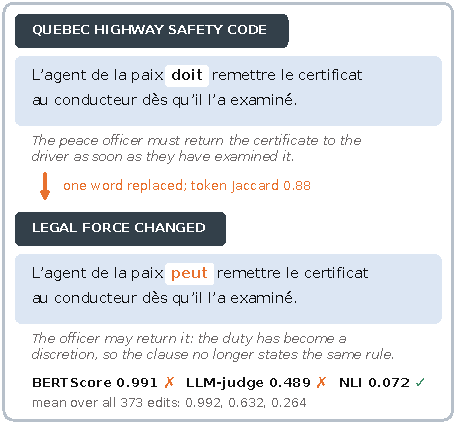
\includegraphics[width=\columnwidth]{figs/teaser_rev.pdf}
\end{figure}

\rev{This article makes four contributions.

\begin{enumerate}\itemsep1pt
\item It states a four-part validation protocol for any scorer of legal meaning
  preservation. The protocol applies to any scoring function and presupposes no
  architecture.
\item It releases \textsc{LexFlip}, a diagnostic set of \numedits\ minimally
  edited Quebec statutory sentences whose legal force has changed and whose
  surface form has hardly changed. Two force-preserving control sets are built
  on the same sentences.
\item It administers the protocol to thirteen untrained scorers: similarity
  metrics, natural language inference, surface features and a prompted large
  language model judge. It also tests a second judge from a different model
  family, and seven fine-tuned regressors that we report separately. Correlation with
  human ratings and sensitivity to a legally decisive edit come apart.
\item It trains metrics against the protocol. The constraint does not transfer
  from the training mixture to the statutory probes.
\end{enumerate}}

\subsection{Related Work}\label{sec:related}

\rev{\paragraph{Evaluating simplification and meaning preservation}
BLEU does not correlate with meaning preservation when a system splits sentences
\cite{sulem2018bleu}. More generally, Alva-Manchego et al.\
\cite{alvamanchego2021unsuitability} show that the agreement of automatic
simplification metrics with human judgments depends on the kind of
simplification and on the quality of the outputs. Legal simplification adds a
further requirement: the legal effect must survive the rewrite
\cite{garimella2022legalsimp}. Our point of departure is the trained
meaning-preservation metric of Beauchemin et al.\ \cite{beauchemin2023meaningbert}
and its legal successor, fitted to \textsc{FrJudge} \cite{beauchemin2025judgebert}.
\textsc{FrJudge} is the only publicly released corpus we know of with human
ratings of legal meaning preservation.

\paragraph{Minimal pairs and behavioural tests}
The diagnostic belongs to a tradition of minimally different inputs.

\begin{itemize}\itemsep1pt
\item Contrast sets \cite{gardner2020contrast} perturb test items in small ways
  that change the label.
\item CheckList \cite{ribeiro2020checklist} separates \emph{directional} tests,
  where an edit should move the output, from \emph{invariance} tests, where it
  should not.
\item PAWS \cite{zhang2019paws} pairs sentences with almost total lexical
  overlap that are not paraphrases.
\item NLI stress tests \cite{naik2018stress} and negation benchmarks
  \cite{hossain2020negation} probe edits like the ones our rules make.
\end{itemize}

For generation metrics, perturbation checklists \cite{sai2021perturbation} and
blind-spot analyses \cite{he2023blindspots} find that embedding-based metrics are
insensitive to negation and to similar errors that change meaning. Chen and Eger
\cite{chen2023menli} show that metrics built on natural language inference
repair much of that gap, and Mujahid et al.\ \cite{mujahid2026stress} run the
complementary experiment for factual consistency in summarization. In
CheckList's terms, \textsc{LexFlip} is a directional test, and the
force-preserving controls of Section~\ref{sec:specmethod} are its invariance
test. Part of our central finding confirms these results for a new language and
register: overlap-based metrics barely react to a high-overlap edit that changes
meaning. Three things are new. The property we hold fixed and move is legal
force, not truth value or sentiment. The validation checks in current use for
legal metrics are satisfiable by construction. And each legal edit is paired with
a specificity control on the same sentence, which the general-domain studies
above do not provide.

\paragraph{Legal NLP and LLM judges}
Entailment over legal text is an established task. COLIEE includes statute
entailment \cite{goebel2024coliee}, and ContractNLI applies document-level
inference to contracts \cite{koreeda2021contractnli}, where negation by exception
is a known difficulty. LegalBench \cite{guha2023legalbench} measures legal
reasoning in large language models. Prompted models now serve as judges
\cite{zheng2023judging}, also in legal evaluation \cite{enguehard2025lemaj}, and
their scores are known to depend on presentation order and wording.
Section~\ref{sec:judge} tests both. We follow Bean et al.\
\cite{bean2025construct} and Pacchiardi et al.\ \cite{pacchiardi2024cleverhans}
on construct validity. For statistics we follow Deutsch et al.\
\cite{deutsch2021statistical}, Steiger \cite{steiger1980tests} and Graham and
Baldwin \cite{graham2014williams}, and for rating distributions Plank
\cite{plank2022variation} and Xu and Jurgens \cite{xu2026disagreement}.}

\section{What Would Validate a Legal Meaning Metric?}\label{sec:protocol}

\rev{The four requirements below apply to any scorer $m(o,s)$ of an original
clause $o$ and a candidate simplification $s$. None of them presupposes an
architecture. Table~\ref{tab:glossary} defines the technical terms that we use
from here on, for readers who come from law rather than from natural language
processing.}

\begin{table}
\centering
\caption{\rev{Terms used in this article.}}\label{tab:glossary}
\small
\rev{\setlength{\tabcolsep}{4pt}
\begin{tabular}{@{}p{0.27\columnwidth}p{0.68\columnwidth}@{}}
\toprule
Term & Meaning \\
\midrule
Metric, scorer & An automatic function that gives a number for how well a simplification $s$ keeps the meaning of an original $o$. \\
Legal force & What a provision does in law: who it binds, whether it obliges or permits, what it covers, and how much. \\
Dissociation & A test item in which two variables that usually move together are separated. Here, surface wording stays fixed and legal force changes, or the reverse. \\
Token Jaccard & The share of distinct words two sentences have in common: $1$ for identical sentences, $0$ for no shared words. \\
Margin & The share of a metric's own identical-to-unrelated range that it uses on a legally decisive edit. Higher is better. \\
Specificity drop & The same quantity for an edit that keeps legal force. The ideal value is $0$. \\
Selectivity & Margin minus specificity drop, on the same sentences. \\
NLI (bidirectional) & Natural language inference: a model gives the probability that one sentence follows from another. We test both directions and keep the lower value. \\
Pearson $r$, Spearman $\rho$ & Correlation of a metric with the human ratings: $1$ is perfect agreement, $0$ is none. $\rho$ uses ranks only. \\
Human ceiling & The correlation one annotator reaches with the mean of the other four. It shows how well a single expert agrees with the panel. \\
Isotonic calibration & A monotone map from a metric's raw score to the $1$--$10$ scale, fitted on training data. It changes the scale and keeps the ranking. \\
Bootstrap interval & A $95\%$ range for a statistic, found by recomputing it on many resamples of the items. \\
\bottomrule
\end{tabular}
}
\end{table}

\rev{\paragraph{R1: a measured ceiling}
A correlation with human judgment means nothing until we know what correlation a
human achieves. A corpus with $k \geq 3$ ratings per item gives this at no cost.
Hold out one rater, correlate that rater's ratings with the mean of the other
$k-1$, and average over the held-out position. That answers the question
\emph{is the metric as good as an expert?} The Spearman--Brown reliability of
the $k$-rater mean answers a different question: \emph{is it as good as the
aggregate label allows?} A metric can sit above the first and below the second
without being superhuman, because predicting an average is easier than being a
rater. The two numbers must also come from the same items and the same kind of
target. Section~\ref{sec:ceiling} computes them in this way.

\paragraph{R2: identical supervision}
Published comparisons put an unsupervised cosine similarity and a fine-tuned
regressor in one table, rescale the similarity by a constant, and report RMSE
for both. A constant rescaling fixes the range but not the location or the shape
of the distribution. A similarity that occupies $[0.7,1.0]$ therefore records a
large RMSE however well it ranks, and the RMSE column measures supervision, not
judgment. We instead fit a monotone map from raw score to the human scale on the
training split alone. Isotonic regression cannot improve a ranking, and rank
statistics move by at most $\isoDeltaRho$.

\paragraph{R3: a trivial-feature control}
Simplifications are usually shorter than their originals, and omission is the
most frequent annotated error. A rubric that deducts one point per identified
error therefore yields a label that the number of deleted words partly predicts.
We require a supervised baseline over surface features alone, fitted under R2.

\paragraph{R4: dissociation}
On naturally occurring pairs, surface form and legal force vary together. The
endpoint checks inherit this confound. Let $s'$ be a perturbation of $s$ with
token Jaccard $J(s,s') \approx 1$ and legal force $L(s') \neq L(s)$. \rev{Let $(a,b)$ be a pair of unrelated
sentences of the same register.} We report the
\emph{margin fraction}
\[
\frac{\overline{m(s,s)} - \overline{m(s,s')}}{\overline{m(s,s)} - \overline{m(a,b)}},
\]
the share of the metric's own identical-to-unrelated range that it spends on a
legally decisive edit. The margin charges a metric against the range it actually
has, not against a nominal $[0,1]$. A metric that treats the edited sentence as
it treats an unrelated one scores $1$. A pure overlap function scores near $0$.
The margin is not the rate at which $(s,s)$ outranks $(s,s')$. That rate is the
weaker quantity, because a metric can rank every item correctly while it moves a
thousandth of its range.

A large margin is necessary but not sufficient. A metric that dropped on
\emph{any} edit would also earn one. We therefore read the margin beside the
same quantity on a control edit $s''$ that leaves legal force unchanged,
$L(s'')=L(s)$. A counterfactual edit isolates the variable of interest only
against such a meaning-preserving control \cite{yang2026compared}. We call the
second quantity the \emph{specificity drop}, with an ideal value of $0$. We call
the difference between the two, on the same source sentences, the
\emph{selectivity}. The dissociation holds for a metric only when the margin is
large \emph{and} the drop is near zero. Two kinds of control matter, and we
build both. The first is a single inert rewrite at the overlap of the legal
edit. The second is a plain-language paraphrase at low overlap, which is what a
real simplifier produces.

The ideal margin is not $1$. A sentence whose obligation became a permission
still concerns the same subject. Nothing requires a metric to place it as far
away as an unrelated statute. No human baseline on \textsc{LexFlip} exists to say
where a competent rater would place it. We therefore read margins comparatively,
across metrics and against each metric's own specificity drop, and not against a
fixed bar.}

\section{Materials and Methods}\label{sec:methods}

\subsection{The \textsc{LexFlip} Diagnostic}\label{sec:lexflip}

\rev{The source sentences come from two Quebec statutes that do not occur in
\textsc{FrJudge}: the Automobile Insurance Act and the Highway Safety Code. Each
sentence receives one minimal edit that changes legal force and leaves the rest
of the sentence intact. We organise the inventory by legal effect, not by
linguistic category. Seven families make up \emph{tier 1}, where the edit
changes who is bound, whether an obligation exists, what is covered, or how
much.

\begin{itemize}\itemsep1pt
\item Modality: \emph{doit} $\leftrightarrow$ \emph{peut}.
\item Party: \emph{l'assur\'e} $\leftrightarrow$ \emph{l'assureur}.
\item Polarity: \emph{ne \dots pas} is dropped.
\item Quantum: an amount or period is multiplied by $10$.
\item Scope: \emph{tous les} $\rightarrow$ \emph{certains}.
\item Time: \emph{avant} $\leftrightarrow$ \emph{apr\`es}.
\item Exception: \emph{sauf si} $\rightarrow$ \emph{si}, \emph{sauf}
  $\rightarrow$ \emph{y compris}, \emph{\`a moins que} $\rightarrow$
  \emph{pourvu que}.
\end{itemize}

\emph{Tier 2} holds the connective shifts (\emph{et} $\leftrightarrow$
\emph{ou}) and the vehicle-class shift (\emph{automobile} $\leftrightarrow$
\emph{v\'ehicule}). We report every result for each tier separately as well.

The diagnostic would fail if a metric could find the edited item because it
reads badly. A conservative French well-formedness check therefore removes every
perturbation that introduces a grammatical artefact. The check flags none of the
$400$ unmodified sources. Of the $400$ sampled sources, $25$ admit no rule, and
for $2$ every candidate edit fails the check. This leaves \numedits\ pairs
(\numeditsTierOne\ in tier 1), with a mean token Jaccard of \meanjaccard\ and
none below \minjaccard. Table~\ref{tab:examples} gives examples, and
Table~\ref{tab:rules} gives the number of items for each rule and tier.

\paragraph{What the labels assert}
The labels are definitional. We assert that an edit changes legal force, and we
did not ask lawyers to rate each item. The strength of that assertion depends on
the rule.

\begin{itemize}\itemsep1pt
\item Modality covers $193$ of the \numedits\ items. Its label rests on the
  Quebec Interpretation Act \cite{interpretationact}. Under it, a thing that
  ``shall'' or ``must'' be done is imperative. A thing that ``may'' be done is
  permissive.
\item Polarity, quantum and time edits change the rule on its face.
\item Party swaps, connectives and the vehicle-class rule are weaker. Their
  effect depends on the provision and on statutory definitions. For example,
  \emph{automobile} is a defined term in the Automobile Insurance Act, so the
  vehicle-class edit changes scope through a definition. It does not reverse a
  rule.
\end{itemize}

Several rules alter legal force without reversing it. An obligation that becomes
a discretion is not the opposite rule, so we speak of a change of force
throughout. The scope rule also has a visible weakness. It maps singular
\emph{tout} and \emph{toute} to \emph{certain} and \emph{certaine}, which gives
unidiomatic statutory French (``\emph{certaine chose}'') on $\nSingular$ items.
We keep the released set unchanged so that every number stays comparable.
Removing those items moves no reported margin by more than $\maxSingularShift$.
Section~\ref{sec:audit} describes the expert audit of a stratified sample.

\paragraph{Probes and normalisation}
For each source $s$ with perturbation $s'$, we score $(s,s)$ and $(s,s')$. The
unrelated probes are \numedits\ separate pairs $(a,b)$. Each pairs a sentence of
the Automobile Insurance Act with a sentence of the Highway Safety Code. The two
share the register but not the content, with a unigram overlap (ROUGE-1 F) of at
most $0.25$. Section~\ref{sec:diagnostic} reports how the margin moves when we
redraw these pairs or change the overlap threshold.

For display, we min--max normalise each metric over all $3\times\numedits$ of
its item-level scores. The \emph{mean} of a probe therefore need not sit at $0$
or $1$. For example, the identical pairs of bidirectional NLI average $0.784$,
because mDeBERTa's entailment probability on identical input varies from item to
item. The margin is a ratio of differences, so this rescaling does not change it.
\emph{Discrimination} is the share of items with $m(s,s) > m(s,s')$ strictly. A
tie therefore counts as a miss, and we report the tie rate beside it.}

\begin{table}
\centering
\caption{\rev{\textsc{LexFlip} examples from seven tier-1 rules, with the edited
span in bold. Each edited sentence shares almost all of its tokens with the
original and changes the legal force of the provision.}}\label{tab:examples}
\small
\rev{\setlength{\tabcolsep}{4pt}
\begin{tabular}{@{}p{0.97\columnwidth}@{}}
\toprule
\emph{peut} $\rightarrow$ \emph{doit} \hfill \emph{tier 1} \\[1pt]
\footnotesize $o$: La Société peut refuser une indemnité, en réduire le montant, en suspendre ou en cesser le paiement dans les cas suivants: 1. \\[1pt]
\footnotesize $s'$: La Société \textbf{doit} refuser une indemnité, en réduire le montant, en suspendre ou en cesser le paiement dans les cas suivants: 1. \\
\midrule
\emph{doit} $\rightarrow$ \emph{peut} \hfill \emph{tier 1} \\[1pt]
\footnotesize $o$: Lorsqu’il n’y a pas de feux pour piétons, un piéton doit se conformer aux feux de circulation. \\[1pt]
\footnotesize $s'$: Lorsqu’il n’y a pas de feux pour piétons, un piéton \textbf{peut} se conformer aux feux de circulation. \\
\midrule
drop \emph{ne \dots pas} \hfill \emph{tier 1} \\[1pt]
\footnotesize $o$: Les feux visés au paragraphe 2\textdegree{} ne sont pas requis pour tout véhicule dont la largeur excède 2,03 mètres. \\[1pt]
\footnotesize $s'$: Les feux visés au paragraphe 2\textdegree{} sont requis pour tout véhicule dont la largeur excède 2,03 mètres. \\
\midrule
\emph{avant} $\leftrightarrow$ \emph{apr\`es} \hfill \emph{tier 1} \\[1pt]
\footnotesize $o$: Elle n’est pas due avant le septième jour qui suit celui de l’accident, sauf dans le cas prévu au troisième alinéa de l’article 57. \\[1pt]
\footnotesize $s'$: Elle n’est pas due \textbf{après} le septième jour qui suit celui de l’accident, sauf dans le cas prévu au troisième alinéa de l’article 57. \\
\midrule
\emph{tous les} $\rightarrow$ \emph{certains} \hfill \emph{tier 1} \\[1pt]
\footnotesize $o$: Le paiement par la Société lui cède tous les droits du réclamant sans restriction. \\[1pt]
\footnotesize $s'$: Le paiement par la Société lui cède \textbf{certains} droits du réclamant sans restriction. \\
\midrule
\emph{assureur} $\rightarrow$ \emph{assur\'e} \hfill \emph{tier 1} \\[1pt]
\footnotesize $o$: L’assureur émet l’attestation d’assurance au plus tard dans les vingt et un jours de la demande d’assurance. \\[1pt]
\footnotesize $s'$: \textbf{L’assuré} émet l’attestation d’assurance au plus tard dans les vingt et un jours de la demande d’assurance. \\
\midrule
\emph{sauf} $\rightarrow$ \emph{y compris} \hfill \emph{tier 1} \\[1pt]
\footnotesize $o$: Deux cyclistes sont autorisés à circuler côte à côte sur une vélorue, sauf s’ils circulent à contresens. \\[1pt]
\footnotesize $s'$: Deux cyclistes sont autorisés à circuler côte à côte sur une vélorue, \textbf{y compris} s’ils circulent à contresens. \\
\bottomrule
\end{tabular}
}
\end{table}

\rev{\subsection{Force-Preserving Controls}\label{sec:specmethod}
We build two control sets on the \textsc{LexFlip} source sentences themselves, so
that every comparison with the legal edit is paired by sentence.

\paragraph{Neutral edits}
A neutral edit keeps the overlap of \textsc{LexFlip} and leaves legal force
unchanged. Each applies one substitution that Quebec statutory drafting treats as
equivalent.

\begin{itemize}\itemsep1pt
\item A subordinator: \emph{lorsque} $\rightarrow$ \emph{quand}.
\item A connective adverb: \emph{toutefois} $\rightarrow$ \emph{cependant},
  \emph{en outre} $\rightarrow$ \emph{de plus}.
\item Self-reference: \emph{le pr\'esent article} $\rightarrow$ \emph{cet
  article}.
\item A referential phrase: \emph{en vertu de} $\rightarrow$ \emph{aux termes
  de}, \emph{conform\'ement \`a} $\rightarrow$ \emph{selon}.
\item A numeral written out: \emph{30 jours} $\rightarrow$ \emph{trente jours}.
\item A rewrite that touches an obligation or prohibition marker and keeps its
  force: \emph{est tenu de} $\rightarrow$ \emph{doit}, \emph{nul ne}
  $\rightarrow$ \emph{personne ne}.
\end{itemize}

The last kind is the hardest test of whether a metric reacts to a modal token or
to the force that the token carries. A neutral edit applies to $\nNeutral$ of the
\numedits\ sources. The mean token Jaccard is $\neutralJaccard$, against
$\meanjaccard$ for \textsc{LexFlip}, and every edit passes the same
well-formedness check.

\paragraph{Paraphrases}
A paraphrase changes the wording a lot and leaves legal force unchanged. This is
what a real simplifier produces. Llama-3.3-70B-Instruct rewrote each source once
in plain French, at temperature $0$. The instruction required it to keep the
parties, modality, conditions, exceptions, deadlines, amounts and
cross-references exactly, and to change the wording as much as possible. We keep
a rewrite only if it meets three conditions. It passes the well-formedness
check, keeps every number of the source, and shares at most $60\%$ of its
tokens with the source. $\nPara$ of the
\numedits\ rewrites pass, with a mean token Jaccard of $\paraJaccard$. Llama is
also one of our judges, so its own scores on this cell may favour its own
wording. The other judge and the untrained metrics do not have this exposure.
Whether a paraphrase really keeps legal force is itself a legal judgment, so the
expert audit below includes a sample of these items.

\subsection{Label Audit}\label{sec:audit}
We audited the definitional labels of the legal edits and of both
controls on a stratified sample of $\nAudit$ items. The sample holds $112$
\textsc{LexFlip} items and $44$ items from each control set. It takes at least
six items per rule, or all items where a rule has fewer. Each item appears with the full article it
comes from, so that cross-references and defined terms are available. The
annotator does not see the rule or the cell, and the items are shuffled. Each
item has four questions.

\begin{enumerate}\itemsep1pt
\item Does the edit change the legal effect?
\item If it does, does it reverse the rule or alter its scope?
\item How severe is the change for a person who relies on the edited text?
\item Is the edited sentence acceptable statutory French?
\end{enumerate}

One Quebec jurist labelled all $\nAudit$ items blind, reading each item beside
its source article and answering the four questions. A single annotator gives no
measure of agreement between jurists. We therefore read the audit as an expert
check on the labels and not as a full validation. We release the blind workbook, the
labelling interface and the answer key so that further jurists can extend it.
Section~\ref{sec:auditresults} presents the results.}

\subsection{Scorers Evaluated}\label{sec:scorers}

\rev{We administer only metrics that handle French, because scoring an
English-only metric on French confounds coverage with quality.
Table~\ref{tab:challenge} names the three families.

\begin{itemize}\itemsep1pt
\item BERTScore \cite{zhang2019bertscore} over CamemBERTv2 and FlauBERT, in F1
  and recall-only variants. Recall targets omission.
\item Four sentence-embedding cosines: LaBSE, multilingual E5-base,
  paraphrase-multilingual-mpnet and Sentence-CamemBERT.
\item Bidirectional natural language inference with mDeBERTa-XNLI
  \cite{laurer2024nli}. A failure of $o \Rightarrow s$ signals hallucination,
  and a failure of $s \Rightarrow o$ signals omission. These are the two most
  frequent categories of the legal error taxonomy.
\end{itemize}

We add token Jaccard and the surface features of R3.}

\subsection{The \textsc{FrJudge} Corpus and Its Reconstruction}\label{sec:corpus}

\rev{The diagnostic answers R4. We answer the other three requirements on
\textsc{FrJudge} \cite{beauchemin2025judgebert}, and then ask whether the two
kinds of evidence agree. \textsc{FrJudge} holds 297 insurance clauses that
\texttt{gpt-4-turbo-2024-04-09} simplified and that five law students rated for
legal meaning on a scale of $1$ to $10$. The public release drops annotator
identity, which makes R1 impossible downstream. We therefore rebuild the corpus
from the raw Prodigy export. The rebuild recovers the five annotators
(pseudonymised as A--E) and reproduces the published pairwise agreement of
$25.96\%$. The same export records the source document of each clause, which the
public release also drops. Section~\ref{sec:grouped} uses it to build a
document-grouped split.

We did not obtain this export privately. The \textsc{FrJudge} authors distribute
it in their own public repository, beside the released corpus and under the same
open licence. It records the annotators' first names, which we never use. Our
loader replaces them with stable pseudonyms on reading, the copy in our
repository is pseudonymised, and we reported the names to the corpus authors.

The splits have $178$, $30$ and $89$ pairs for training, development and test.
We draw them under ten seeds for the unsupervised comparison and under five for
the trained models. We fit the isotonic calibration of R2 on the training split
alone, never on the split that a number comes from.}

\subsection{Prompted Judges}\label{sec:judgemethod}

\rev{A prompted model that receives the annotators' rubric is the natural
competitor to a fine-tuned encoder of 112M parameters. Legal LLM-as-a-judge
protocols are also an active line of work \cite{enguehard2025lemaj}. We score
each pair with \texttt{deepseek-chat} under the \textsc{FrJudge} scale. This is a
ten-point judgment that deducts one point per identified legal error, as the
corpus annotators did \cite{beauchemin2025judgebert}. The published description
does not give the annotators' instructions word for word, so our prompt is a
reconstruction. Each pair goes in its own request, so the judge never sees the
probe condition. We draw $K=5$ samples at temperature $1$ and average them.

We compare three prompt wordings. The first is the \textsc{FrJudge} rubric in
French. The second is the same rubric in English over the same French text. The
third is a bare instruction without the four-type error taxonomy. As a capability control, we run a reasoning model
(\texttt{deepseek-reasoner}) under the same rubric on the same items.
Table~\ref{tab:judgeconfigs} lists every configuration with its prompt, model,
number of samples, item set and calibration. It also names the headline
configuration that the rest of the article quotes. Table~\ref{tab:prompts} gives
the prompts.

Hosted models change behind a fixed name, so we record what we can.
\texttt{deepseek-chat} and \texttt{deepseek-reasoner} are the provider's model
aliases. We drew the responses behind the original experiments no later
than \judgeDateFirst. We drew the responses for the controls added in this
version on \judgeDateRev. Every response is cached, so every number can be recomputed
without the API. Across all configurations, redraws and controls, the DeepSeek
judges received $\judgeCallsTotal$ requests, at an estimated cost of
\$$\judgeCostTotal$.

A judge from one model family cannot show that a finding concerns judges in
general rather than that family. We therefore repeat the headline configuration,
the order control and the force-preserving controls with a second judge. It is
an open-weight model from a different family: Llama-3.3-70B-Instruct with 4-bit
AWQ weights, served with vLLM on one NVIDIA A100 80GB GPU. It receives the same prompts, with $K=5$
and temperature $1$. Its replies are parsed from the prompt's JSON instruction,
as for the reasoning model, because grammar-constrained decoding failed with
this model. Finally, we test whether a judge's treatment of an edit depends on
which sentence it sees as the original. We score every \textsc{LexFlip} edit a
second time with the two sentences exchanged.}

\subsection{Trained Metric Variants}\label{sec:variants}

\rev{The protocol so far audits scorers that already exist. It also has two
consequences for how to fit a new scorer, and we test both. The first follows
from R1. The gold label is the mean of five ratings whose median spread is
\medianRange\ points. A scalar regressor fitted to that mean must predict a
quantity that no annotator asserted, and the loss rewards a prediction near the
centre. The second follows from R4. If a diagnostic identifies a deficiency, the
obvious response is to train against it.

The seven configurations share an encoder (CamemBERTv2-base), the splits, the
schedule and the seeds. The first five differ only in the target and the loss.
The two augmented configurations (\textbf{DA} and \textbf{DA+LexFlip}) keep the
scalar objective and change the training data.

\begin{itemize}\itemsep2pt
\item \textbf{Scalar}, the conventional objective: mean squared error against
  the mean rating.
\item \textbf{Distributional}: a ten-way head trained with KL divergence against
  the empirical rating histogram, after Uma et al.\ \cite{uma2021learning} and
  Peterson et al.\ \cite{peterson2019human}. The reported score is the
  expectation of the distribution, so it stays comparable. The model also
  exposes the spread.
\item \textbf{Annotator-aware}: five regression heads, one per annotator,
  averaged at inference. The model can then represent the lenient and strict
  populations of Section~\ref{sec:ceiling} separately instead of averaging them
  away.
\item \textbf{Quantile}: a pinball loss \cite{koenker1978regression} at
  $\tau=0.25$. The asymmetry is deliberate. A metric that \emph{overshoots} the
  human rating accepts bad simplifications, and a metric that undershoots is
  only strict. In a legal setting these errors do not cost the same, and a
  quantile objective puts that preference into the loss.
\item \textbf{Multi-task}: the scalar head plus an auxiliary head for the
  annotators' characterisation of the clause, trained against their majority
  vote. The vote covers 17 of the rubric's 18 classes, because the eighteenth
  never has a majority. \textsc{FrJudge} collects these labels and then discards
  them. The published rubric has annotators characterise a clause \emph{before}
  they score it, so the label plausibly carries information about the score.
\item \textbf{DA}: the scalar objective, with the identical/unrelated
  augmentation in current use added to the training mixture.
\item \textbf{DA+LexFlip}: \textbf{DA} plus minimally edited negatives, which
  the rules of Section~\ref{sec:lexflip} generate from \textsc{FrJudge}
  originals. They are disjoint from the diagnostic's own sentences.
\end{itemize}

We compute correlation and RMSE \emph{only} on the human-annotated test split,
never on a split that contains augmentation. This matters. Identical pairs
(label 10) and unrelated pairs (label 1) in an evaluation set inflate the label
variance at the extremes. That raises Pearson $r$ for every metric without any
improvement in judgment. A table that mixes the two shows a clear signature: the
$r$ and the RMSE of a metric improve and worsen together. Here the augmentation
affects training only, and we report the three diagnostic regimes separately as
pass rates.

\rev{We tested this mechanism directly, with no training involved. On each of
the ten test splits, we correlated every untrained scorer with the human label
twice. The first time uses the human items only. The second adds one identical
pair (label $10$) and one unrelated pair (label $1$) per test item, the mixture
of \textsc{DA}. The added pairs raise $r$ by $\augSimGainLo$ to $\augSimGainHi$
for every similarity metric, by $\augNliGain$ for bidirectional NLI and by
$\augJudgeGain$ for the DeepSeek judge. Token Jaccard rises from
$\augJacHuman$ to $\augJacAug$. The length feature, the strongest scorer on
human items, falls from $\augLenHuman$ to $\augLenAug$, so the augmented set
also reverses the ranking. A gap of about $0.2$ between our retrained baseline
and the published correlation is well within this effect. We cannot confirm
that it is the cause without the original evaluation set.}

The augmentation is sized to the training split, which has $178$ human pairs.
\textbf{DA} adds $178$ identical pairs (label $10$) and $178$ unrelated pairs
(label $1$). The mixture therefore has two augmented items per human item.
\textbf{DA+LexFlip} adds $178$ minimally edited negatives (label $1$), for three
augmented items per human item. The unrelated pairs come from the same two
statutes as the diagnostic's unrelated probes. The statutes are absent from
\textsc{FrJudge}, but not from these two training mixtures. In the main grid the
identical pairs and the edited negatives came from all $297$ \textsc{FrJudge}
originals, test items included. The in-distribution experiment of
Section~\ref{sec:training} draws them from the training split alone.

A trained model passes the identical-pair check on an item when it predicts at
least $9.9$ on the $1$--$10$ scale. It passes the unrelated-pair check when it
predicts at most $1.1$. This is the strict reading of ``maximum'' and
``minimum'' that the checks in current use imply. We also report the looser
criteria of $9$ and $2$. For trained models, the \textsc{LexFlip}
discrimination counts an item as correct only when the identical pair scores at
least one point above the edited pair.}

\subsection{Statistical Procedures}\label{sec:stats}

\rev{The unsupervised metrics and the length feature correlate with the
\emph{same} human label on the \emph{same} $297$ items, and with each other. A
two-sample test on Fisher-transformed correlations would therefore be
anticonservative. We use the Williams test
\cite{steiger1980tests,graham2014williams}, which corrects for this dependence,
and we apply Holm's step-down correction across the ten tests. We compute power
for the same dependent design, by simulation at the median observed correlation
between a metric and the length feature ($r=\powerRtwothree$). On a
$\testN$-item test split, a reliable distinction from a metric at $r=0.46$ needs
$r \leq \powerBelow$, with $80\%$ power.

The $297$ items of \textsc{FrJudge} come from only $21$ source forms, and items
from one form are not independent. We therefore report two intervals for corpus
correlations: one from a bootstrap over items, and one from a cluster bootstrap
that resamples source forms. Margins carry percentile bootstrap intervals. These
resample source sentences, keeping the identical and edited scores of each
sentence together, and they resample unrelated probes independently. Every
bootstrap uses $2{,}000$ draws.

We report trained models as means and standard deviations over five seeds, and
unsupervised comparisons over ten. We treat any difference smaller than that
spread as unresolved. A seed fixes both the split and the initialisation. We therefore
also rerun the scalar baseline with the split fixed and the initialisation
varied, and the reverse. This separates the two sources of variance.

A laptop produces every number for the untrained metrics, the trained models and
the DeepSeek judges, end to end. The largest trained model is CamemBERTv2-base
(112M parameters). The open-weight judge is the one exception and needs one 80GB
GPU. Training runs use Apple MPS kernels, which are not bitwise deterministic. A
fixed seed therefore reproduces a run only approximately. Repeat runs of the
scalar configuration at seed $42$ differ in test-set $r$ by several hundredths,
which is comparable to the spread across seeds. A reproduction on CUDA should
give tighter agreement and narrower error bars.}

\subsection{Use of Generative AI}\label{sec:aidisclosure}

\rev{Generative AI has two distinct roles in this work. We separate them because
only one of them is a result. As an \emph{object of study},
\texttt{deepseek-chat}, \texttt{deepseek-reasoner} and Llama-3.3-70B-Instruct
are scored as prompted judges under the protocol of
Section~\ref{sec:judgemethod}. Llama-3.3-70B-Instruct also generated the
paraphrase control set of Section~\ref{sec:specmethod}, and
\texttt{gpt-4-turbo-2024-04-09} produced the simplifications in \textsc{FrJudge}
before this work began. Separately, the author used a large language model
assistant to rephrase passages of the manuscript for clarity. No AI system is an
author. The author designed the study and verified every reported number
against the released result files. The author takes full responsibility for the
content of this article, including any part produced with the help of such a
tool.}

\begin{table*}
\centering
\caption{\rev{\textsc{LexFlip}. \emph{ident.} and \emph{unrel.} are the mean
identical-pair and unrelated-pair scores. We min--max normalise over all
$3\times\numedits$ item scores of each metric, so these means need not equal
$1$ and $0$. \emph{discrim.} is the share of items with $m(s,s) > m(s,s')$
strictly. \emph{ties} is the share with $m(s,s) = m(s,s')$, and ties count as
misses.
\emph{Margin} is the share of the identical-to-unrelated range spent on the
legal edit, with a $95\%$ bootstrap interval. The last two columns give it
separately for the \numeditsTierOne\ tier-1 and $63$ tier-2 items.}}\label{tab:challenge}
\footnotesize
\rev{\setlength{\tabcolsep}{3.5pt}
\begin{tabular}{lrrrrrcrr}
\toprule
Metric & ident. & unrel. & discrim.\% & ties\% & margin & $95\%$ CI & tier 1 & tier 2 \\
\midrule
NLI-bidirectional (min) & 0.784 & 0.010 & 93.3 & 0.0 & 0.670 & [0.626, 0.721] & 0.760 & 0.228 \\
NLI-bwd (no omission) & 0.784 & 0.042 & 77.2 & 0.0 & 0.473 & [0.418, 0.532] & 0.554 & 0.075 \\
NLI-fwd (no hallucination) & 0.784 & 0.043 & 77.7 & 0.0 & 0.424 & [0.375, 0.476] & 0.472 & 0.189 \\
Judge: DeepSeek-chat ($K{=}5$) & 1.000 & 0.006 & 86.3 & 13.7 & 0.370 & [0.336, 0.402] & 0.413 & 0.158 \\
Judge: Llama-3.3-70B ($K{=}5$) & 1.000 & 0.004 & 90.3 & 9.7 & 0.106 & [0.098, 0.116] & 0.112 & 0.078 \\
surface: token Jaccard & 1.000 & 0.089 & 99.2 & 0.8 & 0.079 & [0.075, 0.083] & 0.082 & 0.065 \\
LaBSE & 1.000 & 0.292 & 100.0 & 0.0 & 0.039 & [0.036, 0.043] & 0.042 & 0.027 \\
BERTScore-FlauBERT & 1.000 & 0.393 & 100.0 & 0.0 & 0.035 & [0.032, 0.038] & 0.035 & 0.034 \\
mE5-base & 1.000 & 0.266 & 100.0 & 0.0 & 0.034 & [0.031, 0.036] & 0.038 & 0.012 \\
Para-mUSE-mpnet & 1.000 & 0.312 & 100.0 & 0.0 & 0.028 & [0.024, 0.034] & 0.033 & 0.005 \\
Sentence-CamemBERT & 1.000 & 0.316 & 100.0 & 0.0 & 0.024 & [0.021, 0.027] & 0.026 & 0.015 \\
BERTScore-CamemBERTv2-Recall & 1.000 & 0.240 & 100.0 & 0.0 & 0.023 & [0.021, 0.025] & 0.023 & 0.020 \\
BERTScore-CamemBERTv2 & 1.000 & 0.193 & 100.0 & 0.0 & 0.022 & [0.021, 0.024] & 0.023 & 0.021 \\
surface: $-|\,|s|-|o|\,|$ & 1.000 & 0.718 & 11.3 & 88.7 & 0.011 & [0.008, 0.014] & 0.013 & 0.000 \\
\bottomrule
\end{tabular}
}
\end{table*}

\section{Results}\label{sec:results}

\subsection{Similarity Metrics Fail the Dissociation}\label{sec:diagnostic}

\rev{Every similarity-based metric fails, and it fails almost completely
(Table~\ref{tab:challenge}). The seven embedding and BERTScore variants spend
between $\simMarginLo$ and $\bertMargin$ of their working range on an edit that
changes the law. BERTScore over CamemBERTv2 places the edited sentence at
$0.982$. The original sits at $1.000$ and an unrelated statute at $0.193$. Token
Jaccard, at $0.079$, is in the same regime. This is the expected result: these
metrics are overlap functions, as Section~\ref{sec:protocol} predicts. Their
discrimination rates do not help either. All seven rank the identical pair
first on $100\%$ of items, but by a margin too small to support any decision.

Bidirectional NLI does not fail. It spends $\maxMargin$ of its range on the edit
($95\%$ CI $[\nliMarginLo, \nliMarginHi]$) and ranks $93.3\%$ of items
correctly. It also places the edited sentence nearer the unrelated pair than the
identical one. The prompted judge spends $\judgeMargin$ ($[\judgeMarginLo,
\judgeMarginHi]$). It ties the identical and the edited pair on $\judgeTies\%$
of items, mostly by giving both the maximum score. The intervals do not overlap
between any two of the three groups.

The result does not depend on the probe details. We redrew the unrelated pairs
$\nUnrelDraws$ times, with overlap thresholds from $0.10$ to $0.35$. The NLI
margin stays between $\nliUnrelLo$ and $\nliUnrelHi$, and every similarity
metric stays between $\simUnrelLo$ and $\simUnrelHi$. The result also holds on each tier
separately. On tier 2, every margin is smaller: NLI falls from $\nliMarginTone$
to $\nliMarginTtwo$ and the judge to $\judgeMarginTtwo$. Tier-2 edits change
scope rather than reverse a rule, so this is the expected direction. The
length feature's near-zero margin holds by construction, because a one-word
substitution hardly changes length. We report it as a check on the harness,
not as evidence. Figure~\ref{fig:challenge} shows the same result. For every
similarity metric the edited sentence sits hard against the identical pair, at
the wrong end of the metric's own range.}

\begin{figure}
\centering
\caption{\textsc{LexFlip}. \rev{For each metric, the grey bar is its full
working range. It spans the score on an unrelated pair (dark circle) to the score
on an identical pair (blue circle).} The red diamond is where it places a sentence whose
legal force \rev{a single word has changed}. A metric that measured legal
meaning would put the diamond \rev{well to the left}. Every similarity-based
metric puts it at the right, hard against the identical pair. Only the four
scorers above the dashed rule, the three NLI variants and the prompted judge,
move it appreciably. \rev{Metric names are abbreviated.
Table~\ref{tab:challenge} gives them in full, and the margin column is repeated
at the right here.}}\label{fig:challenge}
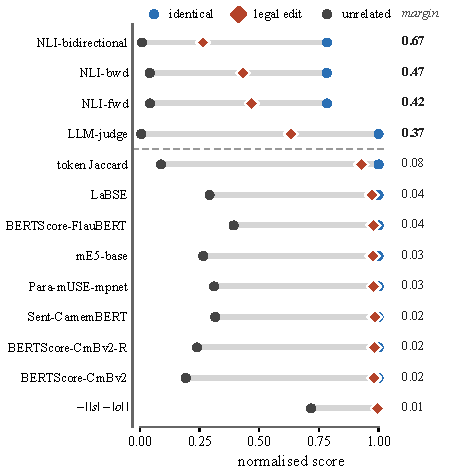
\includegraphics[width=\columnwidth]{figs/challenge.pdf}
\end{figure}

\paragraph{The existing checks would have excluded it}
\rev{NLI's identical score sits at $0.784$, and this is not a normalisation
artefact. In raw terms mDeBERTa gives a sentence paired with itself a mean
entailment probability of $\nliIdentRaw$. Only $\nliIdentPass\%$ of items clear
the $99\%$ bar that the identical-pair convention requires, against $100\%$ for
every BERTScore and embedding metric. The convention would therefore
\emph{disqualify} the metric that best tracks legal force. Every overlap
function saturates on identical input by construction, so saturation is easy to
build. Report it, but do not filter on it.}

\subsection{Which Edits Are Detected}\label{sec:rules}

\rev{An average over all thirteen scorers hides the informative result, because
ten of the thirteen read overlap. Table~\ref{tab:rules} therefore reports each
rule for each scorer family. The similarity family spends at most $0.05$ of its
range on any rule. The two other families differ by rule, and the differences
are legally informative.

\begin{itemize}\itemsep2pt
\item NLI is close to the ideal on dropped negation ($0.985$) and on
  \emph{doit} $\rightarrow$ \emph{peut} ($0.981$). It is strong on quantum,
  time and exception edits.
\item NLI is weak where the edit changes \emph{who} the rule concerns. It spends
  $0.119$ on \emph{assureur} $\rightarrow$ \emph{assur\'e}, $0.054$ on the
  vehicle class, and about $0.26$ on the connectives.
\item The DeepSeek judge is the reverse on parties. It spends $0.581$ on
  \emph{assureur} $\rightarrow$ \emph{assur\'e}, but only $0.137$ on
  \emph{tous les} $\rightarrow$ \emph{certains} and $0.221$ on \emph{peut}
  $\rightarrow$ \emph{doit}.
\item Both families treat the two directions of the modality rule differently:
  NLI spends $0.981$ and $0.703$, the judge $0.590$ and $0.221$.
  Section~\ref{sec:judge} tests the judge's asymmetry directly.
\end{itemize}

Several cells rest on few items. \emph{Assur\'e} $\rightarrow$
\emph{assureur} has three, and time, exception and party have nine to eleven
each. The ordering of rules is therefore descriptive. Two observations are
durable: the similarity family reacts to no rule, and NLI and the judge fail on
different rules. A legal
metric built from either would inherit a specific blind spot.}

\begin{table}
\centering
\caption{\rev{\textsc{LexFlip} margin by rule and scorer family, with tiers
marked. \emph{Similarity} is the mean margin of the seven embedding and
BERTScore metrics (their range in the last row). \emph{NLI-bi} is
bidirectional NLI, and the judge columns use the headline configuration. A
margin of $1$ would mean the scorer treats the edited sentence as it treats an
unrelated one.}}\label{tab:rules}
\small
\rev{\resizebox{\columnwidth}{!}{\setlength{\tabcolsep}{3.5pt}
\begin{tabular}{lrrrrr}
\toprule
Rule & $n$ & similarity & NLI-bi & DeepSeek & Llama \\
\midrule
\multicolumn{6}{l}{\emph{Tier 1}} \\
\emph{peut} $\rightarrow$ \emph{doit} & 111 & 0.027 & 0.703 & 0.221 & 0.088 \\
\emph{doit} $\rightarrow$ \emph{peut} & 82 & 0.029 & 0.981 & 0.590 & 0.110 \\
\emph{tous les} $\rightarrow$ \emph{certains} & 42 & 0.038 & 0.574 & 0.137 & 0.107 \\
drop \emph{ne \dots pas} & 21 & 0.050 & 0.985 & 0.984 & 0.222 \\
amount $\times 10$ & 21 & 0.045 & 0.761 & 0.403 & 0.154 \\
\emph{assureur} $\rightarrow$ \emph{assur\'e} & 11 & 0.020 & 0.119 & 0.581 & 0.112 \\
\emph{sauf (si)} $\rightarrow$ \emph{si}, \emph{y compris} & 10 & 0.036 & 0.755 & 0.754 & 0.112 \\
\emph{avant} $\leftrightarrow$ \emph{apr\`es} & 9 & 0.021 & 0.846 & 0.567 & 0.112 \\
\emph{assur\'e} $\rightarrow$ \emph{assureur} & 3 & 0.019 & -0.033 & 0.395 & 0.037 \\
\midrule
\multicolumn{6}{l}{\emph{Tier 2}} \\
\emph{et} $\rightarrow$ \emph{ou} & 27 & 0.021 & 0.262 & 0.133 & 0.093 \\
\emph{ou} $\rightarrow$ \emph{et} & 26 & 0.015 & 0.258 & 0.221 & 0.062 \\
\emph{automobile} $\leftrightarrow$ \emph{v\'ehicule} & 10 & 0.026 & 0.054 & 0.065 & 0.083 \\
\midrule
\textbf{All} & 373 & 0.022--0.039 & 0.670 & 0.370 & 0.106 \\
\bottomrule
\end{tabular}
}}
\end{table}

\rev{\subsection{Force-Preserving Edits}\label{sec:specificity}

Table~\ref{tab:specificity} gives the second half of the dissociation. For each
scorer, it reports the \textsc{LexFlip} margin on the sources that carry a
control, the drop on each control, and the selectivity.

\paragraph{Neutral edits}
The similarity metrics drop by $\simNeutralDropLo$ to $\simNeutralDropHi$ of
their range on a neutral edit. That is as much as they drop on a legal edit, so
their selectivity is $\simNeutralSelLo$ to $\simNeutralSelHi$. They react to a
change of wording, and the change of law adds nothing. Bidirectional NLI does
not drop at all (drop $\nliNeutralDrop$, $95\%$ CI $[\nliNeutralDropLo,
\nliNeutralDropHi]$), so its selectivity is $\nliNeutralSel$
($[\nliNeutralSelLo, \nliNeutralSelHi]$). The DeepSeek judge does not drop
either (drop $\judgeNeutralDrop$, selectivity $\judgeNeutralSel$). Llama does
not drop (drop $\llamaNeutralDrop$), but its margin is small, so its selectivity
is only $\llamaNeutralSel$. The hardest
neutral edits touch a prohibition marker: \emph{nul ne} becomes \emph{personne
ne}. On these, NLI scores the edited pair slightly \emph{above} the identical
pair (drop $\nliNulNe$). For these two families, the large margin is therefore
not a reaction to any edit. It is a reaction to the edit that changes the law.

\paragraph{Paraphrases}
The label audit (Section~\ref{sec:auditresults}) found that only part of the
paraphrase cell keeps legal force, so this cell is read with that caveat.
On the paraphrases, the order reverses. The similarity metrics drop by
$\simParaDropLo$ to $\simParaDropHi$ of their range, more than they drop on a
legal edit. Their selectivity is therefore negative ($\simParaSelLo$ to
$\simParaSelHi$). They penalise a rewrite more than a change of law.
Bidirectional NLI drops by only $\nliParaDrop$ ($95\%$ CI $[\nliParaDropLo,
\nliParaDropHi]$), and its selectivity stays at $\nliParaSel$. NLI therefore
does not reject a low-overlap rewrite merely because the wording changed. The
DeepSeek judge drops by $\judgeParaDrop$, so it penalises rewording to some
degree. Llama drops by $\llamaParaDrop$, but Llama wrote the paraphrases and may
favour its own wording. Because part of this cell changes legal force, these
drops mix a penalty for rewording with a correct response to a change of law.}

\begin{table}
\centering
\caption{\rev{Specificity. \emph{\textsc{LexFlip} margin} is computed on the
sources that carry a neutral edit. \emph{Drop} is the share of the same
identical-to-unrelated range lost on a force-preserving edit (ideal $0$), and
\emph{select.}\ is margin minus drop on the same sources (higher is better).
Neutral edits keep the overlap of \textsc{LexFlip}. Paraphrases have low
overlap.}}\label{tab:specificity}
\footnotesize
\rev{\resizebox{\columnwidth}{!}{\setlength{\tabcolsep}{3.5pt}
\begin{tabular}{lrrrrr}
\toprule
& \textsc{LexFlip} & \multicolumn{2}{c}{neutral edit} & \multicolumn{2}{c}{paraphrase} \\
\cmidrule(lr){3-4}\cmidrule(lr){5-6}
Metric & margin & drop & select. & drop & select. \\
\midrule
NLI-bidirectional (min) & 0.625 & -0.021 & 0.646 & 0.056 & 0.649 \\
NLI-bwd (no omission) & 0.451 & -0.047 & 0.498 & 0.004 & 0.504 \\
NLI-fwd (no hallucination) & 0.390 & -0.056 & 0.446 & -0.124 & 0.569 \\
Judge: DeepSeek-chat ($K{=}5$) & 0.353 & 0.000 & 0.352 & 0.174 & 0.178 \\
Judge: Llama-3.3-70B ($K{=}5$) & 0.104 & 0.001 & 0.104 & 0.028 & 0.078 \\
BERTScore-CamemBERTv2 & 0.018 & 0.022 & -0.004 & 0.466 & -0.442 \\
BERTScore-CamemBERTv2-Recall & 0.018 & 0.023 & -0.005 & 0.485 & -0.461 \\
BERTScore-FlauBERT & 0.029 & 0.034 & -0.005 & 0.562 & -0.525 \\
LaBSE & 0.034 & 0.004 & 0.030 & 0.190 & -0.148 \\
Sentence-CamemBERT & 0.022 & 0.006 & 0.016 & 0.214 & -0.189 \\
Para-mUSE-mpnet & 0.021 & 0.002 & 0.018 & 0.123 & -0.092 \\
mE5-base & 0.030 & 0.007 & 0.023 & 0.311 & -0.275 \\
\bottomrule
\end{tabular}
}}
\end{table}

\rev{\subsection{What the Label Audit Shows}\label{sec:auditresults}

The jurist of Section~\ref{sec:audit} agrees with the definitional
label on $\expTOneAgree$ of $\expTOneN$ tier-1 items and on $\expTTwoAgree$ of
$\expTTwoN$ tier-2 items. Three of the four tier-1 disagreements are a negated modal: \emph{ne peut}
becomes \emph{ne doit}, and both still state a prohibition. The fourth is a
generator error.
The tier-2 disagreements are connectives, where \emph{et} and \emph{ou} in a list
of applicable articles often leave the rule unchanged. This confirms the
concern that connective edits are weak labels. Of the $\expYes$ edits judged to
change legal force, only $\expReverse$ reverse the rule. The others change its
scope, which is why we speak of a change of force and not of a reversal.

Three further findings bear on how to read the results. First, $\expLexUnidiom$
of the $\expLexN$ edited sentences were judged unidiomatic or ungrammatical,
against $\expCtrlUnidiom$ of the $\expCtrlN$ controls. The scope and vehicle-class rules
account for most of them, so the well-formedness check was weaker than intended.
Second, the annotation exposed generator errors. A search of all \numedits\
items finds $\nBugs$ of them. Seven vehicle-class edits produce \emph{une
automobile routier}. Two party edits fire on the verb \emph{s'assurer}
(\emph{s'\^etre assur\'e} becomes \emph{s'\^etre assureur}). Two time edits fire
on a word that is not temporal (the spatial \emph{avant}, and
\emph{ci-apr\`es}). One modality edit fires inside \emph{qu'il peut le faire}. Removing these items moves no
margin by more than $\maxBugShift$. Third, the neutral edits hold up: all
$\expNeuN$ sampled neutral edits were judged to keep legal force. The paraphrases
do not. Only $\expParAgree$ of $\expParN$ were judged to keep legal force,
$\expParChange$ were judged to change it, and $\expParUncertain$ were uncertain.
One paraphrase replaces \emph{responsabilit\'e solidaire} with \emph{conjointe},
a different liability regime under Quebec civil law. The paraphrase cell is
therefore not a clean force-preserving control, and a drop on it is partly a
correct response.}

\subsection{Disagreement and the Human Ceiling}\label{sec:ceiling}

\rev{Krippendorff's $\alpha$ for legal meaning is $0.104$ under the
\emph{nominal} coefficient, which is the one usually reported for this corpus. It
is $\alphaOrd$ under the \emph{ordinal} coefficient, which suits an ordered
scale \cite{krippendorff2004content}. Table~\ref{tab:agreement} gives all three
annotation dimensions, and our nominal values reproduce the published ones. We
compute both coefficients with the same library on the same reliability matrix,
so only the distance function explains the difference between $0.104$ and
$\alphaOrd$.

The disagreement that remains after this correction is structural. The
annotators form two stable populations: B, C and D average $\lenientMean$, and A
and E average $\strictMean$. \pctSpreadSix\ of pairs span at least $6$ points
(Figure~\ref{fig:disagree}). The mean of the five ratings has a standard
deviation of $\labelSd$, and a regressor that predicts the middle does well on
such a target. Correlating each annotator with the mean of the other four gives
a ceiling of $\ceilR$ (RMSE $\ceilRmse$). The held-out annotators range from
$0.524$ to $0.680$ (Table~\ref{tab:ceiling}).} \rev{A metric that exceeds
this ceiling is not superhuman.A metric that exceeds
this ceiling is not superhuman. The bound for predicting the five-rater mean is
that mean's own reliability, $\sbRel$ by Spearman--Brown, so a metric can
approach $\sqrt{\sbRel}=\sbSqrt$.

The ceiling above uses all $297$ items, while metric correlations use
$\testN$-item test splits and the five-rater mean. Those two numbers are not
directly comparable. We therefore also compute both on the same terms. On each of
the ten test splits, we correlate each held-out annotator with the mean of the
other four. We also correlate each calibrated metric with those same four-rater
means. On this basis the ceiling is $\ceilTest$. The surface ridge reaches
$\ridgeRfour$, the length feature $\lenRfour$, the prompted judge
$\judgeRfour$, and the best semantic metric (BERTScore over FlauBERT)
$\flauRfour$. The like-for-like comparison therefore confirms both statements
below: the ridge sits at the ceiling, and the judge exceeds it.}

\begin{table}
\centering
\caption{Krippendorff's $\alpha$ on \textsc{FrJudge}. Legal meaning is an
ordinal ten-point scale, for which the nominal coefficient is not the
appropriate measure. \emph{prev.}\ is the value reported by Beauchemin et al.\
\cite{beauchemin2025judgebert}.}\label{tab:agreement}
\small
\setlength{\tabcolsep}{4pt}
\begin{tabular}{lrrr}
\toprule
Dimension & \multicolumn{2}{c}{Krippendorff's $\alpha$} & Reported \\
\cmidrule(lr){2-3}
 & nominal & appropriate & prev. \\
\midrule
Simplicity level & 0.183 & 0.183 & 0.18 \\
Characterization & 0.552 & 0.552 & 0.55 \\
Legal meaning & 0.104 & \textbf{0.325} & 0.10 \\
\bottomrule
\end{tabular}
\end{table}

\begin{table}
\centering
\caption{Leave-one-annotator-out ceiling on \textsc{FrJudge} ($n=297$). A
single expert predicts the consensus of the other four at $r=\ceilR$, and the
best-agreeing pair of annotators reaches $r=\bestPairR$.}\label{tab:ceiling}
\small
\setlength{\tabcolsep}{4pt}
\begin{tabular}{lrrr}
\toprule
Held-out & $r$ (95\% CI) & $\rho$ & RMSE \\
\midrule
A & 0.524 [0.44, 0.60] & 0.551 & 3.93 \\
B & 0.569 [0.48, 0.65] & 0.586 & 3.05 \\
C & 0.680 [0.60, 0.75] & 0.725 & 2.75 \\
D & 0.601 [0.52, 0.67] & 0.557 & 3.08 \\
E & 0.612 [0.55, 0.67] & 0.679 & 3.56 \\
\midrule
\textbf{Mean (ceiling)} & \textbf{0.597} & 0.620 & 3.27 \\
Best pair (C-D) & 0.606 & -- & -- \\
Mean pairwise & 0.462 & -- & -- \\
\bottomrule
\end{tabular}
\end{table}

\begin{figure*}
\centering
\caption{Disagreement in \textsc{FrJudge}. \rev{(a) The five annotators form two
populations. B, C and D (blue) rate legal preservation about three points higher
than A and E (red) across the whole corpus. (b) Sorted within-item range. The
median item spans \medianRange\ points of a ten-point scale. (c) A single
annotator predicts the consensus of the other four at $r=\ceilR$ (bar). The
whiskers give the range over the five held-out annotators. The best-agreeing
pair reaches $r=\bestPairR$.}}\label{fig:disagree}
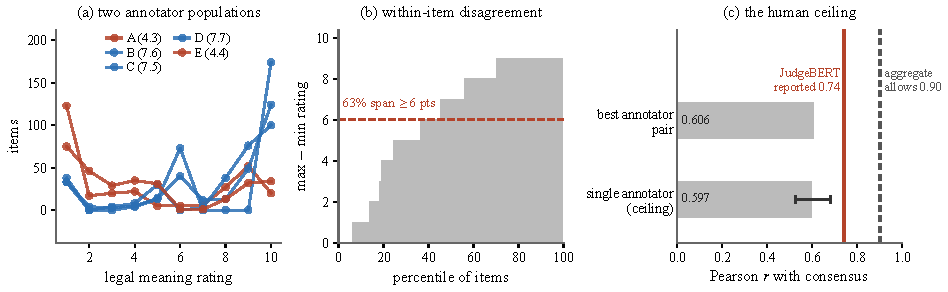
\includegraphics[width=\textwidth]{figs/disagreement.pdf}
\end{figure*}

\begin{table*}
\centering
\caption{Calibrated comparison on the \textsc{FrJudge} test split ($\testN$
items), mean over 10 seeds. \rev{RMSE$_{\text{raw}}$ is the decimal-scaling protocol
in current use. RMSE$_{\text{cal}}$ fits an isotonic map on the training split.
We compute $r$ and $\rho$ after calibration. The map is monotone, so it leaves
$\rho$ almost unchanged (at most $\isoDeltaRho$). It shifts $r$ by up to
$\isoDeltaR$.}}\label{tab:baselines}
\small
\setlength{\tabcolsep}{4pt}
\begin{tabular}{lrrrrr}
\toprule
Metric & $r$ & $\rho$ & RMSE$_{\text{raw}}$ & RMSE$_{\text{cal}}$ & over\% \\
\midrule
\multicolumn{6}{l}{\emph{Unsupervised, French-capable}}\\
BERTScore-CamemBERTv2 & 0.291$_{\pm0.09}$ & 0.326 & 2.62 & 2.36 & 49.3 \\
BERTScore-CamemBERTv2-Recall & 0.352$_{\pm0.12}$ & 0.398 & 2.59 & 2.30 & 47.2 \\
BERTScore-FlauBERT & 0.482$_{\pm0.08}$ & 0.459 & 2.16 & 2.12 & 49.4 \\
LaBSE & 0.409$_{\pm0.06}$ & 0.402 & 2.33 & 2.21 & 47.2 \\
Sentence-CamemBERT & 0.296$_{\pm0.05}$ & 0.287 & 2.68 & 2.31 & 49.3 \\
Para-mUSE-mpnet & 0.252$_{\pm0.08}$ & 0.266 & 2.88 & 2.35 & 47.2 \\
mE5-base & 0.358$_{\pm0.08}$ & 0.356 & 2.52 & 2.26 & 48.0 \\
NLI-fwd (no hallucination) & 0.368$_{\pm0.06}$ & 0.352 & 3.85 & 2.25 & 49.3 \\
NLI-bwd (no omission) & 0.340$_{\pm0.09}$ & 0.355 & 3.70 & 2.28 & 46.9 \\
NLI-bidirectional (min) & 0.395$_{\pm0.07}$ & 0.405 & 3.74 & 2.22 & 46.6 \\
\midrule
\multicolumn{6}{l}{\emph{Trivial surface features}}\\
$-|\,|s|-|o|\,|$ (length difference) & 0.641$_{\pm0.04}$ & 0.624 & 3.25 & 1.85 & 47.0 \\
Token Jaccard & 0.303$_{\pm0.06}$ & 0.331 & 3.34 & 2.34 & 48.0 \\
Length ratio & 0.580$_{\pm0.05}$ & 0.560 & 3.43 & 1.97 & 49.1 \\
Surface-Ridge (10 features, supervised) & 0.621$_{\pm0.05}$ & 0.588 & 1.89 & 1.89 & 45.8 \\
\midrule
\multicolumn{6}{l}{\emph{Prompted LLM judge}}\\
LLM-judge (deepseek-chat, k=5) & 0.755$_{\pm0.05}$ & 0.753 & 2.93 & 1.57 & 43.9 \\
\midrule
\textbf{Human ceiling} (one annotator) & \textbf{0.597} & 0.620 & -- & 3.27 & -- \\
\bottomrule
\end{tabular}
\end{table*}

\subsection{Identical Supervision, and a Trivial Control}\label{sec:baselines}

\rev{Calibration removes most of the RMSE gap that uncalibrated comparisons
record (Table~\ref{tab:baselines}). The metrics were not as far from human
judgment as such tables suggest. They were on a different scale. A ridge over
word counts and token overlap reaches $r=\surfR$. This is at the human ceiling
and above every semantic metric we test, of which the best reaches $r=0.482$.
Only two scorers beat the ridge, and neither is semantic: the prompted judge
below, and the bare length difference at $r=0.641$.

Under the Williams test, each of the ten unsupervised neural metrics is
significantly \emph{worse} than the length feature ($t$ between $2.61$ and
$6.33$, Table~\ref{tab:significance}). All ten
comparisons survive Holm's correction for ten tests (largest adjusted $p =
\holmMaxP$). The Williams test assumes independent items, and \textsc{FrJudge}
items cluster in $21$ source forms. A cluster bootstrap over forms is the
stricter test. Under it, the length feature's lead stays resolved for
$\nClusterSig$ of the ten metrics. It is not resolved for BERTScore over
FlauBERT (difference $\lenMinusFlau$, $95\%$ CI $[\lenMinusFlauLo,
\lenMinusFlauHi]$) or for BERTScore-CamemBERTv2 recall. The length feature's own
correlation has a cluster interval of $[\lenRclLo, \lenRclHi]$, against
$[\lenRitLo, \lenRitHi]$ over items. We therefore claim the ordering for most
metrics, not for the two best ones.

The result says less about the corpus than about what the \emph{annotation}
rewards. The rubric reduces the score once per identified error, and the most
frequent error type, omission, goes with a shorter simplification.}

\begin{table}
\centering
\caption{Williams tests against the trivial length baseline
$\ell = -|\,|s|-|o|\,|$. \rev{Over all $297$ items, $\ell$ reaches $r=0.613$
with the human label $h$.} $r(m,\ell)$ is each metric's correlation with the length
feature itself, the dependence the test corrects for. Positive $t$ favours
$\ell$. \rev{$p_{\text{Holm}}$ is adjusted for the ten tests. The last column is
the $95\%$ cluster-bootstrap interval, over the $21$ source forms, for
$r(\ell,h)-r(m,h)$.}}\label{tab:significance}
\footnotesize
\rev{\resizebox{\columnwidth}{!}{\setlength{\tabcolsep}{4pt}
\begin{tabular}{lrrrrc}
\toprule
Neural metric $m$ & $r(m,h)$ & $t$ & $p$ & $p_{\text{Holm}}$ & cluster CI \\
\midrule
BERTScore-CamemBERTv2 & 0.344 & 5.05 & $<$0.001 & $<$0.001 & [0.038, 0.397] \\
BERTScore-CamemBERTv2-Recall & 0.396 & 4.43 & $<$0.001 & $<$0.001 & [0.009, 0.318] \\
BERTScore-FlauBERT & 0.484 & 2.61 & 0.010 & 0.010 & [-0.026, 0.289] \\
LaBSE & 0.424 & 3.66 & $<$0.001 & $<$0.001 & [0.040, 0.269] \\
Sentence-CamemBERT & 0.222 & 6.33 & $<$0.001 & $<$0.001 & [0.041, 0.472] \\
Para-mUSE-mpnet & 0.225 & 6.32 & $<$0.001 & $<$0.001 & [0.178, 0.513] \\
mE5-base & 0.318 & 5.40 & $<$0.001 & $<$0.001 & [0.101, 0.426] \\
NLI-fwd (no hallucination) & 0.320 & 5.66 & $<$0.001 & $<$0.001 & [0.133, 0.462] \\
NLI-bwd (no omission) & 0.307 & 5.36 & $<$0.001 & $<$0.001 & [0.177, 0.396] \\
NLI-bidirectional (min) & 0.365 & 4.68 & $<$0.001 & $<$0.001 & [0.108, 0.335] \\
\bottomrule
\end{tabular}
}}
\end{table}

\subsection{The Prompted Judges}\label{sec:judge}

\begin{table*}
\centering
\caption{\rev{Every prompted-judge configuration in this article. \emph{Items}
is \emph{all} for the full \textsc{FrJudge} corpus and all \numedits\
\textsc{LexFlip} probes. It is \emph{sub} for the fixed $100$-edit subsample,
with its identical and unrelated probes. We ran the capability and prompt
comparisons on this subsample to keep the reasoning model affordable. \emph{Cal.}\ marks
isotonic calibration under R2, fitted on each training split. The headline row
is the configuration quoted elsewhere in the article. Rows on the subsample are
comparable with each other, not with the full-set rows.}}\label{tab:judgeconfigs}
\footnotesize
\rev{\setlength{\tabcolsep}{3pt}
\begin{tabular}{lllcccrr}
\toprule
Configuration & prompt & model & $K$ & items & cal. & $r$ & margin \\
\midrule
\textbf{Headline} & rubric, FR & deepseek-chat & 5 & all & yes & 0.755 & 0.370 \\
Redraw & rubric, FR & deepseek-chat & 5 & all & yes & 0.726 & 0.372 \\
Uncalibrated & rubric, FR & deepseek-chat & 5 & all & no & 0.719 & -- \\
Single sample & rubric, FR & deepseek-chat & 1 & sub & yes & 0.619 & 0.425 \\
Reasoner & rubric, FR & deepseek-reasoner & 1 & sub & yes & 0.580 & 0.320 \\
Prompt v1 & rubric, FR & deepseek-chat & 2 & sub & yes & 0.687 & 0.421 \\
Prompt v2 & rubric, EN & deepseek-chat & 2 & sub & yes & 0.727 & 0.573 \\
Prompt v3 & bare, FR & deepseek-chat & 2 & sub & yes & 0.758 & 0.687 \\
Second family & rubric, FR & Llama-3.3-70B & 5 & all & yes & 0.709 & 0.106 \\
\bottomrule
\end{tabular}
}
\end{table*}

\rev{Table~\ref{tab:judgeconfigs} lists every configuration. The headline
configuration (the French rubric, \texttt{deepseek-chat}, $K=5$, all items,
calibrated) reaches $r=\judgeR_{\pm\judgeRsd}$ under R2. This is above the
length feature and above our ceiling, and an independent redraw gave
$\repRcalTwo$. On \textsc{LexFlip}, the identical pair scores $\judgeIdent$
and the unrelated pair $\judgeUnrel$. It is therefore flawless on the two
checks that overlap can satisfy. It then gives a clause whose legal force has
changed $\judgeEdit$ out of ten, a margin of $\judgeMargin$. Margins and
correlations from the subsample rows are not comparable with these full-set
values.

The rubric, not the model, limits the margin. With the model fixed, the margin
rises from $\promptMarginLo$ under the rubric-faithful prompt to
$\promptMarginHi$ under a bare instruction without the four-type taxonomy. A
redraw moves it by $0.002$. The correlation rises too, from $\promptRubricR$ to
$\promptBareR$. The rubric reduces the score \emph{once per identified error}.
The judge therefore counts a change of legal force as one incoherence, and the
penalty stays near the top of the scale. A reasoning model does not help. Under the same
rubric and items, \texttt{deepseek-reasoner} gives $r=\reasonerR$ against
$\chatKoneR$, and a margin of $\reasonerMargin$ against $\chatKoneMargin$, at
matched sampling. The shortfall is not a matter of the model thinking harder.

\paragraph{A second model family}
Llama-3.3-70B-Instruct under the headline configuration reaches $r=\llamaRcal$
($\pm\llamaRcalSd$) on \textsc{FrJudge}. On \textsc{LexFlip} it scores the
identical pair at $\llamaIdentical$, the edited pair at $\llamaLexflip$ and the
unrelated pair at $\llamaUnrelated$. Its margin is $\llamaMargin$
(Table~\ref{tab:challenge}). The two families agree on the endpoints and
differ on the edit. Both give every identical pair the top score and almost
every unrelated pair a score near the bottom. Llama, however, scores the edited
pair close to the identical pair. Its margin is less than a third of the
DeepSeek margin, although its correlation with the human ratings stays high.
Llama is therefore the clearest single case of the dissociation. It tracks the
human ratings closely and barely reacts to a change in the law.

\paragraph{The modality asymmetry}
On the full set, DeepSeek gives \emph{doit} $\rightarrow$ \emph{peut} a mean of
$\dsAsymFwdWeaken$ and \emph{peut} $\rightarrow$ \emph{doit} a mean of
$\dsAsymFwdStrengthen$. The gap holds in every configuration, from
$\asymGapLo$ to $\asymGapHi$. It is tempting to read this gap as the judge
tracking legal severity. That reading does not survive two objections. First,
whether a change from obligation to discretion is more or less severe depends
on whose position one takes. A discretion is a gain for the party it frees and a
loss for the party it protected. Second, the gap could follow the direction of
change \emph{as presented} rather than anything legal. We tested the second
objection directly. We scored every edit again with the two sentences exchanged,
so that a \emph{doit} $\rightarrow$ \emph{peut} item reads as \emph{peut}
$\rightarrow$ \emph{doit}. Under the exchange, the \emph{doit}-source items
score $\dsAsymSwWeaken$ and the \emph{peut}-source items $\dsAsymSwStrengthen$.
The gap falls from $\dsAsymFwdGap$ to $\dsAsymSwGap$ points. It does not
reverse. Part of the asymmetry follows the order of presentation. The other part
follows the items: sentences that state an obligation keep a low score whichever
version comes first. Llama shows a much smaller gap: $\llamaAsymFwdGap$ points
in the original order and $\llamaAsymSwGap$ under the exchange. It scores almost
every edit near the top of the scale. Its gap does not reverse
either. We therefore
report the asymmetry as a property of these judges that a deployment must
measure. We do not interpret it as legal severity.

\paragraph{The judge as a sixth annotator}
The judge rates on the annotators' scale, so we can place it inside the panel
and not only beside the metrics. Its mean rating is $\judgeMeanRating$. \rev{The two annotator groups average $\strictMean$ and
$\lenientMean$, and the individual annotators average $4.33$ to $7.72$. The
judge is therefore more lenient than any human and far less dispersed.} Yet its mean correlation with the five
annotators is $\judgeHumanR$, higher than the mean human-to-human correlation
of $\humanHumanR$. Adding it as a sixth coder nonetheless \emph{lowers} ordinal
$\alpha$ from $\alphaOrd$ to $\judgeAlphaPanel$. It tracks the consensus without
belonging to the distribution. It is far more consistent with its own five
samples than the humans are with each other ($\alpha=\judgeAlphaSelf$ against
$\alphaOrd$). Averaging the samples matters: correlation with the human mean
rises from $\judgeKone$ at $K=1$ to $\judgeKfive$ at $K=5$. Its explanations
show the same pattern. On identical pairs it reports an error in
$\judgeErrIdent\%$ of samples. On \textsc{LexFlip} it reports some error in
$\judgeErrEdit\%$, and it names \emph{incoh\'erence}, the correct type for this
edit, in $\judgeErrIncoh\%$.

\paragraph{Combining the judge with NLI}
We tried six rules for combining the judge with bidirectional NLI. Every
calibration and every weight was fitted on the \textsc{FrJudge} training split
by correlation alone, so \textsc{LexFlip} never entered a fit. No rule beats
both parents on both axes. The best, a weighted blend at $w=\hybridW$, reaches
$r=\hybridR$ and a margin of $\hybridMargin$. Its correlation gain over the
judge ($0.007$) is smaller than the variation between two redraws of the judge
($0.029$). Its margin stays below that of NLI alone ($\maxMargin$). We report
this as a negative result and do not propose the blend as a metric.}

\begin{table*}
\centering
\caption{\rev{The judge prompts. The headline configuration uses v1. Each pair
is sent in its own request, $K$ times, and the integer score is read from the
JSON reply.}}\label{tab:prompts}
\scriptsize
\rev{\setlength{\tabcolsep}{4pt}
\begin{tabular}{@{}p{0.15\textwidth}p{0.81\textwidth}@{}}
\toprule
\textbf{System (v1, v3)} & Vous êtes juriste, spécialiste du droit québécois des assurances et de la rédaction législative. Vous évaluez si une reformulation simplifiée d'une clause préserve exactement sa portée juridique. \\
\midrule
\textbf{User, v1 (headline)} & \parbox[t]{0.80\textwidth}{\raggedright Voici une clause originale et sa version simplifiée.\\ \phantom{x}\\ CLAUSE ORIGINALE:\\ \emph{[original clause]}\\ \phantom{x}\\ VERSION SIMPLIFIÉE:\\ \emph{[simplified version]}\\ \phantom{x}\\ Évaluez UNIQUEMENT la préservation du sens juridique: la version simplifiée dit-elle exactement ce que dit l'originale sur le plan du droit? Ignorez complètement la lisibilité, le style et la simplicité -- ils sont évalués séparément.\\ \phantom{x}\\ Barème (échelle ordinale de 1 à 10):\\ - Partez de 10 (portée juridique identique).\\ - Retirez un point par erreur juridique identifiée, parmi:\\   * OMISSION: un élément juridiquement opérant de l'originale a disparu (condition, exclusion, délai, montant, partie liée, exception).\\   * HALLUCINATION: la version simplifiée ajoute un contenu juridique absent de l'originale.\\   * INCOHÉRENCE: la version simplifiée contredit l'originale (modalité, polarité, partie, quantum, portée).\\   * CONFUSION: la version simplifiée rend la règle juridiquement ambiguë ou inintelligible alors que l'originale ne l'était pas.\\ - 1 = le sens juridique n'est pas préservé du tout (règle inversée, autre règle,\\   ou contenu sans rapport).\\ \phantom{x}\\ Répondez uniquement par un objet JSON, sans texte autour:\\ {"erreurs": [{"type": "...", "detail": "..."}], "score": <entier de 1 à 10>}} \\
\midrule
\textbf{User, v3 (bare)} & \parbox[t]{0.80\textwidth}{\raggedright Voici une clause originale et sa version simplifiée.\\ \phantom{x}\\ CLAUSE ORIGINALE:\\ \emph{[original clause]}\\ \phantom{x}\\ VERSION SIMPLIFIÉE:\\ \emph{[simplified version]}\\ \phantom{x}\\ Sur une échelle de 1 à 10, dans quelle mesure la version simplifiée préserve-t-elle le sens juridique de la clause originale? 10 = portée juridique identique, 1 = sens juridique pas préservé du tout. Ignorez la lisibilité et le style.\\ \phantom{x}\\ Répondez uniquement par un objet JSON, sans texte autour:\\ {"erreurs": [], "score": <entier de 1 à 10>}} \\
\midrule
\textbf{v2} & The v1 rubric translated into English, over the same French clauses (system prompt in English). Full text in the repository, \texttt{src/llm\_judge.py}. \\
\bottomrule
\end{tabular}
}
\end{table*}

\begin{table*}
\centering
\caption{\rev{Trained metrics, mean over 5 seeds, evaluated on the
human-annotated test split only. \emph{over\%} is the share of test items on
which the model predicts above the human label. \emph{ident.\ pass} is the share
of identical statutory probes predicted at $\geq 9.9$, and \emph{unrel.\ pass}
the share of unrelated probes predicted at $\leq 1.1$, on the $1$--$10$ scale.
\textsc{LexFlip} false acceptance is the share of edited pairs still scored
$\geq 7$ (``accurate'' under the published rubric). The margin is the quantity
of Section~\ref{sec:protocol}. It is shown as `--' where a model places the
identical and unrelated probes within one point of each other. A model with no
working range has none to spend on the edit. Pass rates and
over\% are percentages.}}\label{tab:models}
\small
\setlength{\tabcolsep}{4pt}
\begin{tabular}{lrrrrrrrr}
\toprule
Model & $r$ & $\rho$ & RMSE & over\% & ident.\ & unrel.\ & \multicolumn{2}{c}{\textsc{LexFlip}} \\
\cmidrule(lr){8-9}
 &  &  &  &  & pass & pass & false-acc.\ & margin \\
\midrule
JudgeBERT-Scalar (baseline) & 0.542$_{\pm0.08}$ & 0.280 & 2.48 & 25.4 & 0 & 0 & 0 & -- \\
JudgeBERT-Dist (soft labels) & 0.572$_{\pm0.03}$ & 0.578 & 1.99 & 42.9 & 0 & 0 & 69 & 0.015 \\
JudgeBERT-Annot (5 heads) & 0.534$_{\pm0.05}$ & 0.585 & 3.47 & 12.6 & 0 & 0 & 0 & -- \\
JudgeBERT-Quantile (tau=.25) & 0.553$_{\pm0.06}$ & 0.377 & 3.28 & 9.9 & 0 & 0 & 0 & -- \\
JudgeBERT-MT (+charact.) & 0.519$_{\pm0.06}$ & 0.232 & 2.51 & 26.3 & 0 & 0 & 0 & -- \\
\midrule
JudgeBERT-DA & 0.192$_{\pm0.25}$ & 0.112 & 2.31 & 42.5 & 0 & 77 & 18 & 0.019 \\
JudgeBERT-DA+LexFlip & 0.122$_{\pm0.10}$ & 0.174 & 2.60 & 35.3 & 0 & 69 & 0 & 0.051 \\
\midrule
\emph{NLI-bidirectional} (untrained) & 0.395 & 0.405 & 2.22 & 46.6 & 1 & -- & -- & \emph{0.670} \\
\textbf{Human ceiling} & \textbf{0.597} & 0.620 & 3.27 & -- & -- & -- & -- & -- \\
\bottomrule
\end{tabular}
\end{table*}

\subsection{What Training Against the Protocol Buys}\label{sec:training}

\rev{Table~\ref{tab:models} reports the grid of Section~\ref{sec:variants}. The
first result is negative. Five configurations differ only in
target and loss. None of them moves the correlation by more than the scalar
baseline's own spread across seeds ($\pm0.082$). That spread is itself far smaller than the
difference of about a quarter of a correlation point that an $\testN$-item split
can resolve. The two augmented configurations are the exception, and they lose
correlation (see below). Most of the seed spread comes from initialisation.
With the split fixed, the standard deviation of $r$ across
$\seedNInit$ initialisations is $\seedSdInit$. With the initialisation fixed, it
is $\seedSdSplit$ across $\seedNSplit$ splits.

The differences that survive are in the other columns. The distributional head
is much steadier than the scalar head ($\pm0.029$ against $\pm0.082$ over the
same five seeds). It reaches the best RMSE in the table ($1.99$) and about
doubles the rank correlation ($\rho=0.578$ against $0.280$). A target that
carries the shape of the rating distribution, and not only its mean, should
have this effect. The quantile head does what it was asked to do. It overshoots
the human label on $9.9\%$ of test items, against $25.4\%$ for the scalar head,
the lowest rate of any model here. Its correlation is unchanged ($0.553$ against
$0.542$), but its RMSE rises from $2.48$ to $3.28$. A model trained at
$\tau=0.25$ predicts below the mean by design. A loss can therefore encode the
risk asymmetry of a legal setting, at a measurable cost in RMSE.

\paragraph{Why the trained models fail the identical-pair check}
Every model in Table~\ref{tab:models} scores $0\%$ on the identical-pair check.
This includes the two augmented models, although their training mixture contains
identical pairs. The augmented models pass the unrelated check on $77\%$ and
$69\%$ of probes, and the other models on none. Two explanations are possible.
Under the first, the identical probes are statutory sentences and the training
identical pairs are \textsc{FrJudge} clauses. Passing would then require a
change of source document. Under the second, a regressor trained toward the label mean
rarely predicts $9.9$ on any input, whatever its source. To separate the two, we
retrained the scalar and augmented models with augmentation drawn from the
training split only. We then tested them on identical pairs built from held-out
\textsc{FrJudge} originals (Table~\ref{tab:indist}). Neither explanation
survives in its simple form. On held-out \textsc{FrJudge} originals, the scalar
model scores identical pairs at $\indScalarIdent$ and unrelated pairs at
$\indScalarUnrel$, and no identical pair reaches either bar. A change of source
document cannot explain this, because these pairs come from the training
distribution. Compression toward the mean cannot explain it either, because a
compressed model would still rank identical pairs above unrelated ones. The
scalar model does not separate them at all. It appears to predict from
properties of the clauses, not from the relation between them. The augmented
models do separate the two endpoints ($\indDaIdent$ against $\indDaUnrel$ for
\textsc{DA}). They still score an edited original as high as the identical pair
($\indDaEdit$), so their margin on held-out originals is $\indDaMargin$.

The diagnostic shows the same pattern. \textsc{DA+LexFlip}, trained on minimally
edited negatives, reaches a margin of $0.051$ on the statutory probes, against
$\maxMargin$ for untrained bidirectional NLI. Its negatives come from
\textsc{FrJudge} originals and its probes from statutes. Table~\ref{tab:indist}
also gives its margin on edits of held-out \textsc{FrJudge} originals. That
margin is $\indDalfMargin$. The model fails on new items of the kind it trained
on, so its failure is not only a transfer failure between corpora.

The augmented mixtures also show the clearest effect in the table.
\textsc{DA} loses $0.350$ of correlation against the scalar baseline, and
\textsc{DA+LexFlip} loses $0.420$, on five seeds out of five in both cases.
\textsc{DA} varies by $\pm0.254$ across seeds and reaches $r=-0.188$ on one of
them.

One column needs care. \textsc{LexFlip} false acceptance is the share of edited
pairs that still score $\geq 7$, so it depends on where a model puts its
predictions overall. The distributional head's $69\%$ reflects a head that
scores high in general: its identical probes average $7.22$. The $0\%$ of the
scalar heads reflects models that score low on everything, not models that
reject the edit.}

\begin{table*}
\centering
\caption{\rev{Identical-pair and \textsc{LexFlip} checks for the scalar and
augmented models, retrained with augmentation drawn from the training split only
(mean over seeds). \emph{Held-out \textsc{FrJudge} originals} are test-split
originals paired with themselves, and edited by the \textsc{LexFlip} rules for
the margin. \emph{Statutory probes} are the probes of Table~\ref{tab:models}.
\emph{ident.}\ and \emph{unrel.}\ are the mean predictions on identical and
unrelated pairs (scale $1$--$10$). $\geq$9.9 and $\geq$9 are the shares of
identical pairs at or above each bar, in percent. The margin is shown as `--' when the model's identical and unrelated
means are less than one point apart.}}\label{tab:indist}
\footnotesize
\rev{\setlength{\tabcolsep}{3pt}
\begin{tabular}{lrrrrrrrrrr}
\toprule
& & \multicolumn{5}{c}{held-out \textsc{FrJudge} originals} & \multicolumn{4}{c}{statutory probes} \\
\cmidrule(lr){3-7}\cmidrule(lr){8-11}
Model & seeds & ident. & unrel. & $\geq$9.9 & $\geq$9 & margin & ident. & $\geq$9.9 & $\geq$9 & margin \\
\midrule
Scalar & 5 & 4.58 & 4.78 & 0 & 0 & -- & 5.17 & 0 & 0 & -- \\
DA & 5 & 6.40 & 4.44 & 0 & 0 & 0.00 & 5.05 & 0 & 0 & 0.01 \\
DA+LexFlip & 5 & 5.70 & 4.85 & 0 & 0 & 0.02 & 4.41 & 0 & 0 & 0.02 \\
\bottomrule
\end{tabular}
}
\end{table*}

\subsection{What Survives a Change of Document}\label{sec:grouped}

\rev{A meta-evaluation that never changes the source document cannot separate
legal sensitivity from familiarity with a form. A random split lets clauses from
the same insurance form appear in both training and test, and insurance forms
are highly templated. We therefore rerun the scalar baseline and the two
augmented mixtures on a document-grouped split, in which no source document
crosses the boundary. The grouped split matches the random split in size, pair
for pair. The other four configurations differ from the baseline in what they
predict, not in what they can exploit about a source form. They therefore face
the same leakage.

The comparison does not resolve. The scalar baseline's correlation falls from
$0.542$ on the random split to $0.454$ on the grouped one. That drop of $0.088$
goes in the direction that leakage would predict, but it does not survive
inspection. The per-seed differences are $+0.169$, $-0.097$, $-0.416$, $-0.182$
and $+0.086$. Two of the five seeds therefore \emph{improve} under the harder
split, and the grouped spread ($\pm0.143$) is wider than the gap itself. The two
augmented mixtures move by $-0.002$ and $+0.026$, which is to say not at all.
As a control, the untrained NLI reference fits nothing and should not care how
the corpus is split. It moves from $0.395$ to $0.391$. The two splits are
therefore otherwise comparable, and the variance above belongs to the models,
not to the split.

We therefore do not claim that document-level leakage inflates these
correlations. Our claim is narrower and, we think, more useful to anyone who
plans a successor corpus. \textsc{FrJudge} is too small and too concentrated to
answer the question. Its 297 pairs come from only 21 source forms, and the three
largest forms hold $71\%$ of them. The largest form alone is $37\%$ of the
corpus. That is more than the $30\%$ test quota, so the form always falls in
training. The grouped test split therefore always comes from the $188$ pairs
that remain. At that size, the variation from seed to seed swamps the effect. A
corpus that must support an out-of-domain claim needs its documents spread far
more evenly. This is the part of the design we would change first.}

\subsection{Stratifying by Length Change}\label{sec:buckets}

\rev{If a metric's correlation comes mostly from items where the simplification
is much shorter, the metric detects deletion, not a change of law.
Table~\ref{tab:buckets} reports Pearson $r$ inside each tercile of
$|\,|s|-|o|\,|$. Within a tercile the length signal is roughly constant. A metric
that keeps its correlation there uses something other than deletion, and a
metric whose correlation collapses was reading length. This is a weaker form of
the dissociation logic of Section~\ref{sec:lexflip}. It holds a confound roughly
fixed by conditioning, not exactly fixed by construction.}

\begin{table}
\centering
\caption{\rev{Correlation with the human label \emph{within} terciles of the
absolute length change. For the length feature and the three unsupervised
metrics, every column uses all $297$ items, and the \emph{all} column equals
the full-corpus value. For the surface ridge and the trained JudgeBERT-Scalar,
every column pools the out-of-fold test predictions over seeds. A tercile
removes most of the length variance. A metric that measures legal meaning should
therefore lose far less correlation there than one that measures deletion.}}\label{tab:buckets}
\small
\setlength{\tabcolsep}{4pt}
\begin{tabular}{lrrrr}
\toprule
& \multicolumn{3}{c}{$r$ within tercile} & \\
\cmidrule(lr){2-4}
Metric & small & medium & large & all \\
\midrule
$-|\,|s|-|o|\,|$ & 0.243 & 0.165 & 0.585 & 0.613 \\
BERTScore-FlauBERT & 0.198 & 0.449 & 0.413 & 0.484 \\
LaBSE & 0.174 & 0.532 & 0.240 & 0.424 \\
NLI-bidirectional & 0.058 & 0.269 & 0.291 & 0.365 \\
Surface-Ridge & 0.118 & 0.305 & 0.540 & 0.620 \\
JudgeBERT-Scalar & 0.042 & 0.149 & 0.602 & 0.496 \\
\bottomrule
\end{tabular}
\end{table}

\rev{The result qualifies Section~\ref{sec:baselines} in a way that cuts against
our own argument, so we state it carefully. The length feature's correlation is
mostly a \emph{between}-tercile effect. Over the corpus it reaches $0.613$. Inside the small and medium
terciles it falls to $0.243$ and $0.165$ ($95\%$ CIs $[\lenBucketLoSmall,
\lenBucketHiSmall]$ and $[\lenBucketLoMedium, \lenBucketHiMedium]$). Among items with a similar length change, the length
change says little. It recovers to $0.585$ only in the tercile where the
simplification is much shorter, which is where deletion is there to detect. The
neural metrics have the opposite profile. In the medium tercile, BERTScore over
FlauBERT holds $0.449$ ($[\flauMedLo, \flauMedHi]$) against $0.484$ pooled, and
LaBSE reaches $0.532$ ($[\labseMedLo, \labseMedHi]$) against $0.424$ pooled. The
intervals are wide, about $100$ items per tercile, so these within-tercile
contrasts are suggestive rather than precise. The surface ridge follows the raw
length feature tercile by tercile, as expected if it is mostly a length model
with extra terms. The small tercile is hard for every scorer. We read this as a
floor effect: when the two sentences have nearly the same length, none of these
signals has much to work with.

The fair reading is therefore narrower than ``legal meaning preservation is
length preservation''. Length dominates the corpus-level ranking, and a
comparison without a length control credits a metric with what belongs to that
confound. But the neural metrics do not read \emph{only} length. Where the
length signal is weakest, they hold up, so whatever they read there is not the
length change. Section~\ref{sec:diagnostic} adds that this residual signal is
still not legal sensitivity, because the same metrics hardly move when the law
changes at fixed length. The two analyses answer different questions, and a
metric has to pass both.}

\begin{figure}
\centering
\caption{\rev{Correlation against legal sensitivity. Horizontally, calibrated
correlation with the human label, the quantity a conventional comparison
selects on. Vertically, the share of the working range spent on an edit that
changes legal force. Dashed lines mark the thresholds used in the text: the
measured human ceiling ($r=\ceilR$) and a margin of $0.5$. Open markers are the
prompt-variant and blend configurations of Section~\ref{sec:judge}. The
bare-prompt point comes from the $100$-edit subsample.}}\label{fig:dissociation}
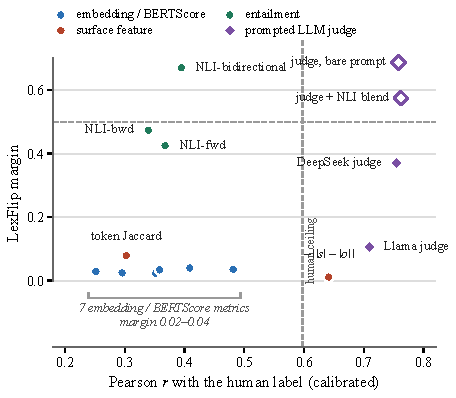
\includegraphics[width=0.82\columnwidth]{figs/dissociation_rev.pdf}
\end{figure}

\subsection{Correlation and Legal Sensitivity Come Apart}\label{sec:dissociation}

\rev{Take the \nDissocAll\ scorers that carry both a calibrated $r$ and a
margin. Over them, the rank correlation between the two is $\rho=\dissocRhoAll$
($95\%$ interval $[\dissocRhoAllLo, \dissocRhoAllHi]$). Seven of those points are
nearly identical similarity metrics, so this interval shows an absence of
resolution, not a demonstrated independence. The extremes are the durable part.
The length feature outscores every semantic metric, and its margin is near zero
by construction. Bidirectional NLI sits mid-table on correlation and reacts most
to the edit.

Figure~\ref{fig:dissociation} marks two thresholds: a correlation at the human
ceiling, and a margin of at least half the working range. None of the thirteen
scorers in the main comparison and none of the trained models passes both. The
region is reachable, however. Two
configurations lie in it. One is the judge under the bare prompt
($r=\promptBareR$, margin $\promptBareMargin$, on the subsample). The other is
the judge--NLI blend ($r=\hybridR$, margin $\hybridMargin$). Neither
was selected on legal sensitivity: the blend was fitted on correlation alone,
and the prompt variants were a robustness check. A comparison that ranks metrics
by correlation would not have found them. That is the practical point. The two
properties do not track each other across the metrics in current use, so
selecting on one does not deliver the other.}

\rev{\section{Discussion}\label{sec:discussion}

The study set out to answer four questions, and the answers are as follows.

\begin{enumerate}\itemsep2pt
\item \textbf{RQ1.} The two checks in current use cannot separate a metric that
  reads legal force from one that reads overlap. Overlap passes both by
  construction.
\item \textbf{RQ2.} The seven similarity metrics barely react to a change of
  legal force. They react just as much to an edit that changes nothing in law.
  Bidirectional NLI and the DeepSeek judge react strongly to the legal edit and
  not at all to the inert one. Llama barely reacts to either. On low-overlap
  paraphrases, the similarity metrics drop more than on a legal edit, and NLI
  barely drops.
\item \textbf{RQ3.} Correlation with human ratings does not predict legal
  sensitivity across the metrics in use. The few configurations that have both
  were found by accident, not by selection.
\item \textbf{RQ4.} Training against the diagnostic did not transfer.
  On held-out items from the training corpus, the trained models still give an
  edited clause the score of an identical one.
\end{enumerate}

\paragraph{What to report}
A metric that claims to measure legal meaning should report three checks, not
two. The identical-pair and unrelated-pair checks show calibration at the
endpoints. \textsc{LexFlip} shows whether the metric moves when the law moves,
and its force-preserving controls show whether it stays still when the law does
not. Overlap satisfies the first two checks and fails the third. A low margin
is therefore a measured deficiency of a metric, not a limit of automatic
evaluation in general. We do not show that the deficiency is easy to fix. Our
one attempt to train it away failed (Section~\ref{sec:training}).

\paragraph{Consequences for practice}
For anyone \emph{building} a metric, the results point to the training
objective. The five configurations that differ only in target and loss move the
correlation by less than seed noise. The two that change the training data lose
correlation. An untrained bidirectional entailment score, the only scorer here
whose objective concerns directional meaning containment, has the largest
margin. It is a hypothesis, not a result, that a metric built on an entailment
objective would keep that sensitivity. The margin of NLI may partly reflect its
familiarity with negation and modality contrasts, and NLI is weak on party
swaps. For anyone \emph{reporting} a metric, R2 and R3 are cheap and change
conclusions. Isotonic calibration removes most of the RMSE gap that uncalibrated
tables attribute to supervision. A length control moves a semantic metric from
``competitive with humans'' to ``below a feature that counts words''. For
anyone \emph{deploying} a metric, the per-rule results are the main warning. NLI
and the judge fail on different rules, and the DeepSeek judge treats the two
directions of the modality rule differently. A deployment has to measure these blind spots
on its own text, because no general score reveals them.

\paragraph{Beyond legal text}
One finding may generalise beyond legal text. A validation protocol built only
from endpoint checks can be satisfied by construction. The repair holds one
variable fixed while it moves the other. It applies to any evaluation where the
property of interest goes with surface form in naturally occurring data. A
second finding is narrower. Training against the diagnostic did not transfer
for one encoder, one corpus and one mixture. This agrees with earlier reports
that counterfactually augmented training data does not reliably improve
generalisation \cite{kaushik2020counterfactual,huang2020counterfactual}. It is
still a hypothesis about diagnostics in training mixtures, not a general result.

\paragraph{For the next corpus}
Three design choices would make the next corpus in this area more useful.
First, spread the source documents evenly enough that a grouped split is
possible. Second, keep a held-out set of minimally edited negatives and
force-preserving controls out of every training mixture. Publish it with the
ratings, so that legal sensitivity can be reported beside correlation. Third,
release a stable pseudonymous identifier for each annotator. This makes a
ceiling measurable downstream. It must be balanced against annotator privacy:
an identifier should carry no name, and timestamps and free-text fields should
be coarsened or reviewed before release. Quebec statutes are enacted in French
and English, so their English versions offer a ready test of whether these
results hold for English drafting.}

\section{Limitations}\label{sec:limits}

\rev{\paragraph{Labels and items}
The \textsc{LexFlip} labels are definitional. The modality rule rests on the
Quebec Interpretation Act, and polarity, quantum and time edits change the rule
on their face. Party, connective and class edits depend on context, and some
edits alter legal force without reversing it. The label audit of
Section~\ref{sec:audit} was done by one jurist, so it gives no agreement
between jurists. A sample cannot certify every item in any case. It found $\nBugs$ generator errors and a
share of unidiomatic edited sentences, which we report rather than remove. The edits are single and generated from templates. Real
simplification errors are more often omissions and lost qualifiers. The
diagnostic is therefore a necessary condition, not a model of real errors. A
system could be tuned to it without acquiring general legal sensitivity. The scope rule
also produces unidiomatic French on $\nSingular$ items, which we report rather
than remove.

\paragraph{Scorers}
Bidirectional NLI's margin may reflect familiarity with the \emph{form} of
negation, modality and quantifier contrasts, rather than sensitivity to their
legal consequence. NLI training data is built around these contrasts
\cite{naik2018stress,hossain2020negation}. The neutral control reduces this concern for edits that
touch a modal token without changing force, but does not remove it. The judge
results rest on two model families and on a rubric we reconstructed from its
published description. Wording alone moves the margin by
$\promptMarginRange$. The open-weight judge also wrote the paraphrase controls,
so its own scores on that cell may favour its own wording.

\paragraph{Scope}
The diagnostic and the corpus comparison run on different text, two statutes
against insurance forms, and answer different questions. No human baseline on
\textsc{LexFlip} exists, so margins are read comparatively. The corpus is one
language and one legal system. The motivating concerns of this article are
partly English and common law, and whether the same dissociation holds for
common-law English drafting is open. The bilingual Quebec statutes are the
natural first test.}

\section{Conclusion}\label{sec:conclusion}

\rev{Legal meaning preservation metrics are validated today by two checks that
lexical overlap satisfies by construction. We proposed a third check that overlap
cannot satisfy, released \textsc{LexFlip} to administer it, and paired it with
controls that change wording but not law. Every similarity-based metric in
current use spends between $\simMarginLo$ and $\bertMargin$ of its working range
on an edit that changes a statutory obligation. It spends about as much on an
edit that changes nothing. Bidirectional NLI spends $\maxMargin$ on the first and
nothing on the second. It is the family that the identical-pair convention
would have excluded. On the only public corpus for this task, a supervised ridge
over word counts matches the measured human ceiling and beats most semantic
metrics. A prompted judge exceeds the ceiling but gives a clause whose legal
force has changed $\judgeEdit$ out of ten. Across the metrics in use,
correlation with human ratings does not predict sensitivity to a change in the
law. Reporting both, with a force-preserving control, is the smallest change
that would make the difference visible.}

\section*{Acknowledgement}\label{acknowledgement}

\rev{An earlier version of this work is available as a preprint on arXiv
(arXiv:2609.05296).} The author thanks the authors of \textsc{FrJudge} for
releasing the corpus and the raw annotation export on which the reconstruction
in Section~\ref{sec:corpus} depends. \rev{The author also thanks the Quebec
jurist who labelled the audit sample.}

\section*{Funding Support}\label{funding-support}

This research received no specific grant from any funding agency in the public,
commercial, or not-for-profit sectors.

\section*{Ethical Statement}\label{ethical-statement}

\rev{The label audit of Section~\ref{sec:audit} was carried out by one Quebec
jurist, who took part voluntarily and is not named. The audit collected no
personal data, and only the item-level labels are released. The study involves
no animal subjects. If further jurists extend the audit, their responses will be
collected on the same terms and reported only in aggregate.

The study reuses an existing annotated corpus, \textsc{FrJudge}, and
pseudonymises its five annotators as A--E throughout. The corpus authors
distribute the raw annotation export publicly, under the same licence as the
corpus. The export records the annotators' first names. We never use or publish
these names. Our code replaces them with pseudonyms on loading, our copy
coarsens per-annotation timestamps to the day, and we reported the issue to the
corpus authors. We also release the pseudonymisation script for anyone who
redistributes a reconstruction.

Beauchemin et al.\ \cite{beauchemin2025judgebert} caution that their metric
informs a practitioner about legal meaning preservation but does not supply a
complete juridical analysis. Our results turn that caution into a rule. A metric
that cannot distinguish \emph{doit} from \emph{peut} must not decide whether a
simplified clause is safe to publish. The appropriate use is triage, the ranking
of clauses for human review, not certification. Nothing in this article is legal
advice. The perturbed sentences we release are deliberate misstatements of Quebec
law. The release labels them as such, and they are not statements of the law.}

\section*{Conflicts of Interest}\label{conflicts-of-interest}

The author declares that he has no conflicts of interest to this work.

\section*{Data Availability Statement}\label{data-availability-statement}

\rev{The data and code that support the findings of this study are openly
available at \url{https://github.com/Nyvora-Vision-Labs/LexFlip}. The repository
contains the following.

\begin{itemize}\itemsep1pt
\item The \textsc{LexFlip} generator, the released item set and the two
  force-preserving control sets.
\item The expert-audit sample, its blind workbook and the key that maps items to
  rules.
\item The scoring harness, the cached responses of every prompted judge, the
  document-grouped splits, and the result files behind every table.
\item A pseudonymised reconstruction of \textsc{FrJudge} from the corpus
  authors' public raw export, with annotator identity (as A--E) and source
  document. We redistribute this file under the licence of the original corpus
  \cite{beauchemin2025judgebert}, with attribution. The corpus itself remains
  available from its authors.
\end{itemize}

The statutory sentences come from the Automobile Insurance Act and the Highway
Safety Code. Every perturbed sentence is a deliberate misstatement of Quebec law,
and the release labels it as such. The code is released under the MIT licence
and the \textsc{LexFlip} items, controls, audit materials and result files under
CC BY 4.0. The \textsc{FrJudge} reconstruction follows the original corpus,
whose paper and repository state CC BY 4.0 and CC BY-NC-SA 4.0 respectively. We
redistribute it under the stricter CC BY-NC-SA 4.0.}

%% The reference list is set flush to the foot of the page: \flushbottom undoes
%% the document-wide \raggedbottom for this last page, and the infinitely
%% stretchable gap between entries lets both columns run to the bottom margin.
\flushbottom
\begingroup
\setlength{\parskip}{0pt}
\AtBeginEnvironment{thebibliography}{\setlength{\itemsep}{0pt plus 1fill}}
%% Revision reference list (src/make_bib_rev.py). APA form, in order of first
%% citation, so the first work cited is [1]. paper/references_revision.md
%% records how each added entry was verified.

\begin{thebibliography}{99}

\bibitem{moffatt2024} %
\textit{Moffatt v.\ Air Canada}, 2024 BCCRT 149 (British Columbia Civil
Resolution Tribunal, 14 February 2024).

\bibitem{magesh2025hallucinationfree} %
Magesh, V., Surani, F., Dahl, M., Suzgun, M., Manning, C. D., \& Ho, D. E.
(2025). Hallucination-free? Assessing the reliability of leading AI legal
research tools. \textit{Journal of Empirical Legal Studies}, \textit{22}(2),
216--242.

\bibitem{beauchemin2023meaningbert} %
Beauchemin, D., Saggion, H., \& Khoury, R. (2023). MeaningBERT: Assessing
meaning preservation between sentences. \textit{Frontiers in Artificial
Intelligence}, \textit{6}, 1223924.

\bibitem{beauchemin2025judgebert} %
Beauchemin, D., Albert-Rochette, M., Khoury, R., \& D\'eziel, P.-L. (2025).
JUDGEBERT: Assessing legal meaning preservation between sentences. In
\textit{Proceedings of the 2025 Conference on Empirical Methods in Natural
Language Processing} (pp.~92--118).

\bibitem{sulem2018bleu} %
Sulem, E., Abend, O., \& Rappoport, A. (2018). BLEU is not suitable for the
evaluation of text simplification. In \textit{Proceedings of the 2018 Conference
on Empirical Methods in Natural Language Processing} (pp.~738--744).

\bibitem{alvamanchego2021unsuitability} %
Alva-Manchego, F., Scarton, C., \& Specia, L. (2021). The (un)suitability of
automatic evaluation metrics for text simplification. \textit{Computational
Linguistics}, \textit{47}(4), 861--889. \url{https://doi.org/10.1162/coli_a_00418}

\bibitem{garimella2022legalsimp} %
Garimella, A., Sancheti, A., Aggarwal, V., Ganesh, A., Chhaya, N., \&
Kambhatla, N. (2022). Text simplification for legal domain: Insights and
challenges. In \textit{Proceedings of the Natural Legal Language Processing
Workshop 2022} (pp.~296--304).

\bibitem{gardner2020contrast} %
Gardner, M., Artzi, Y., Basmov, V., Berant, J., Bogin, B., Chen, S., Dasigi, P.,
et al. (2020). Evaluating models' local decision boundaries via contrast sets.
In \textit{Findings of the Association for Computational Linguistics: EMNLP
2020} (pp.~1307--1323).

\bibitem{ribeiro2020checklist} %
Ribeiro, M. T., Wu, T., Guestrin, C., \& Singh, S. (2020). Beyond accuracy:
Behavioral testing of NLP models with CheckList. In \textit{Proceedings of the
58th Annual Meeting of the Association for Computational Linguistics}
(pp.~4902--4912).

\bibitem{zhang2019paws} %
Zhang, Y., Baldridge, J., \& He, L. (2019). PAWS: Paraphrase adversaries from
word scrambling. In \textit{Proceedings of the 2019 Conference of the North
American Chapter of the Association for Computational Linguistics: Human
Language Technologies} (pp.~1298--1308).

\bibitem{naik2018stress} %
Naik, A., Ravichander, A., Sadeh, N., Rose, C., \& Neubig, G. (2018). Stress test
evaluation for natural language inference. In \textit{Proceedings of the 27th
International Conference on Computational Linguistics} (pp.~2340--2353).

\bibitem{hossain2020negation} %
Hossain, M. M., Kovatchev, V., Dutta, P., Kao, T., Wei, E., \& Blanco, E.
(2020). An analysis of natural language inference benchmarks through the lens
of negation. In \textit{Proceedings of the 2020 Conference on Empirical Methods
in Natural Language Processing} (pp.~9106--9118).

\bibitem{sai2021perturbation} %
Sai, A. B., Dixit, T., Sheth, D. Y., Mohan, S., \& Khapra, M. M. (2021).
Perturbation CheckLists for evaluating NLG evaluation metrics. In
\textit{Proceedings of the 2021 Conference on Empirical Methods in Natural
Language Processing} (pp.~7219--7234).

\bibitem{he2023blindspots} %
He, T., Zhang, J., Wang, T., Kumar, S., Cho, K., Glass, J., \& Tsvetkov, Y.
(2023). On the blind spots of model-based evaluation metrics for text
generation. In \textit{Proceedings of the 61st Annual Meeting of the
Association for Computational Linguistics (Volume 1: Long Papers)}
(pp.~12067--12097).

\bibitem{chen2023menli} %
Chen, Y., \& Eger, S. (2023). MENLI: Robust evaluation metrics from natural
language inference. \textit{Transactions of the Association for Computational
Linguistics}, \textit{11}, 804--825.

\bibitem{mujahid2026stress} %
Mujahid, Z. M., Wright, D., \& Augenstein, I. (2026). Stress testing factual
consistency metrics for long-document summarization. In \textit{Proceedings of
the 64th Annual Meeting of the Association for Computational Linguistics (Volume
1: Long Papers)} (pp.~31914--31933).

\bibitem{goebel2024coliee} %
Goebel, R., Kano, Y., Kim, M.-Y., Rabelo, J., Satoh, K., \& Yoshioka, M. (2024).
Overview and discussion of the Competition on Legal Information,
Extraction/Entailment (COLIEE) 2023. \textit{The Review of Socionetwork
Strategies}, \textit{18}(1), 27--47.

\bibitem{koreeda2021contractnli} %
Koreeda, Y., \& Manning, C. (2021). ContractNLI: A dataset for document-level
natural language inference for contracts. In \textit{Findings of the
Association for Computational Linguistics: EMNLP 2021} (pp.~1907--1919).

\bibitem{guha2023legalbench} %
Guha, N., Nyarko, J., Ho, D. E., R\'e, C., Chilton, A., Narayana, A.,
Chohlas-Wood, A., et al. (2023). LegalBench: A collaboratively built benchmark
for measuring legal reasoning in large language models. \textit{Advances in
Neural Information Processing Systems}, \textit{36} (Datasets and Benchmarks
Track).

\bibitem{zheng2023judging} %
Zheng, L., Chiang, W.-L., Sheng, Y., Zhuang, S., Wu, Z., Zhuang, Y., Lin, Z.,
et al. (2023). Judging LLM-as-a-judge with MT-Bench and Chatbot Arena.
\textit{Advances in Neural Information Processing Systems}, \textit{36}.

\bibitem{enguehard2025lemaj} %
Enguehard, J., Van Ermengem, M., Atkinson, K., Cha, S., Ghosh Chowdhury, A.,
Kallur Ramaswamy, P., Roghair, J., et al. (2025). LeMAJ (Legal LLM-as-a-Judge):
Bridging legal reasoning and LLM evaluation. In \textit{Proceedings of the
Natural Legal Language Processing Workshop 2025} (pp.~318--337).

\bibitem{bean2025construct} %
Bean, A. M., Kearns, R. O., Romanou, A., Hafner, F. S., Mayne, H., Batzner, J.,
Foroutan Eghlidi, N., et al. (2025). Measuring what matters: Construct validity
in large language model benchmarks. \textit{Advances in Neural Information
Processing Systems}, \textit{38}, 19868--19949.

\bibitem{pacchiardi2024cleverhans} %
Pacchiardi, L., Tesic, M., Cheke, L. G., \& Hern\'andez-Orallo, J. (2024).
Leaving the barn door open for Clever Hans: Simple features predict LLM
benchmark answers. \textit{arXiv preprint arXiv:2410.11672}.

\bibitem{deutsch2021statistical} %
Deutsch, D., Dror, R., \& Roth, D. (2021). A statistical analysis of
summarization evaluation metrics using resampling methods.
\textit{Transactions of the Association for Computational Linguistics},
\textit{9}, 1132--1146.

\bibitem{steiger1980tests} %
Steiger, J. H. (1980). Tests for comparing elements of a correlation matrix.
\textit{Psychological Bulletin}, \textit{87}(2), 245--251.

\bibitem{graham2014williams} %
Graham, Y., \& Baldwin, T. (2014). Testing for significance of increased
correlation with human judgment. In \textit{Proceedings of the 2014 Conference
on Empirical Methods in Natural Language Processing (EMNLP)} (pp.~172--176).

\bibitem{plank2022variation} %
Plank, B. (2022). The ``problem'' of human label variation: On ground truth in
data, modeling and evaluation. In \textit{Proceedings of the 2022 Conference on
Empirical Methods in Natural Language Processing} (pp.~10671--10682).

\bibitem{xu2026disagreement} %
Xu, Y., \& Jurgens, D. (2026). Beyond consensus: Perspectivist modeling and
evaluation of annotator disagreement in NLP. \textit{arXiv preprint
arXiv:2601.09065}.

\bibitem{yang2026compared} %
Yang, Z., Levy, M., Goldberg, Y., \& Wallace, B. C. (2026). Compared to what?
Baselines and metrics for counterfactual prompting. \textit{arXiv preprint
arXiv:2605.01048}.

\bibitem{interpretationact} %
\textit{Interpretation Act}, CQLR c I-16, s 51 (Quebec).

\bibitem{zhang2019bertscore} %
Zhang, T., Kishore, V., Wu, F., Weinberger, K. Q., \& Artzi, Y. (2020).
BERTScore: Evaluating text generation with BERT. In \textit{International
Conference on Learning Representations}.

\bibitem{laurer2024nli} %
Laurer, M., van Atteveldt, W., Casas, A., \& Welbers, K. (2024). Less
annotating, more classifying: Addressing the data scarcity issue of supervised
machine learning with deep transfer learning and BERT-NLI. \textit{Political
Analysis}, \textit{32}(1), 84--100.

\bibitem{uma2021learning} %
Uma, A. N., Fornaciari, T., Hovy, D., Paun, S., Plank, B., \& Poesio, M. (2021).
Learning from disagreement: A survey. \textit{Journal of Artificial Intelligence
Research}, \textit{72}, 1385--1470.

\bibitem{peterson2019human} %
Peterson, J. C., Battleday, R. M., Griffiths, T. L., \& Russakovsky, O. (2019).
Human uncertainty makes classification more robust. In \textit{Proceedings of
the IEEE/CVF International Conference on Computer Vision (ICCV)}
(pp.~9616--9625).

\bibitem{koenker1978regression} %
Koenker, R., \& Bassett, G., Jr. (1978). Regression quantiles.
\textit{Econometrica}, \textit{46}(1), 33--50.

\bibitem{krippendorff2004content} %
Krippendorff, K. (2019). \textit{Content analysis: An introduction to its
methodology}. SAGE. \url{https://doi.org/10.4135/9781071878781}

\bibitem{kaushik2020counterfactual} %
Kaushik, D., Hovy, E., \& Lipton, Z. C. (2020). Learning the difference that
makes a difference with counterfactually-augmented data. In
\textit{International Conference on Learning Representations}.

\bibitem{huang2020counterfactual} %
Huang, W., Liu, H., \& Bowman, S. R. (2020). Counterfactually-augmented SNLI
training data does not yield better generalization than unaugmented data. In
\textit{Proceedings of the First Workshop on Insights from Negative Results in
NLP} (pp.~82--87).

\end{thebibliography}

\endgroup

\end{document}
